\documentclass[12pt,a4paper,fontset=windows]{ctexart}

% === 页面设置 ===
\usepackage[top=2.54cm,bottom=2.54cm,left=2.8cm,right=2.8cm]{geometry}
\usepackage{setspace}
\onehalfspacing  % 1.5 倍行距

% === 字体设置 ===
% ctex 默认使用 Windows 字体（宋体、黑体、楷体、仿宋）
\ctexset{
    section/format = \centering\zihao{3}\heiti,          % 章标题：黑体三号居中
    subsection/format = \zihao{4}\heiti,                  % 节标题：黑体四号
    subsubsection/format = \zihao{-4}\heiti,              % 小节标题：黑体小四
}

% === 常用宏包 ===
\usepackage{amsmath,amssymb,amsthm}
\usepackage{graphicx}
\usepackage{booktabs}
\usepackage{multirow}
\usepackage{float}
\usepackage{caption}
\usepackage{subcaption}
\captionsetup{labelsep=space}  % "图 1 xxx" 而非 "图 1: xxx"
\usepackage[hidelinks]{hyperref}
\usepackage{cleveref}
\usepackage{algorithm2e}
\usepackage{enumitem}
\usepackage{tabularx}
\usepackage{longtable}
\usepackage{placeins}
\usepackage{needspace}
\usepackage{tocloft}
\renewcommand{\cftsecfont}{\fontsize{10.5}{12.5}\selectfont\bfseries}
\renewcommand{\cftsecpagefont}{\fontsize{10.5}{12.5}\selectfont\bfseries}
\renewcommand{\cftsubsecfont}{\fontsize{10.5}{12.5}\selectfont}
\renewcommand{\cftsubsecpagefont}{\fontsize{10.5}{12.5}\selectfont}
\setlength{\cftbeforesecskip}{5pt}
\setlength{\cftbeforesubsecskip}{0pt}
\setlength{\cftaftertoctitleskip}{16pt}

% === TikZ（仅用于架构图/流程图）===
\usepackage{tikz}
\usetikzlibrary{arrows.meta,positioning,shapes.geometric,fit,calc}
% 注意：pgfplots 仅作为备用，数据图表应使用 \includegraphics 引用 matplotlib 生成的 PDF
\usepackage{pgfplots}
\pgfplotsset{compat=1.18}

% === 引用格式 GB/T 7714 ===
\usepackage[super,sort&compress]{gbt7714}

% === 页眉页脚 ===
\usepackage{fancyhdr}
\pagestyle{fancy}
\fancyhf{}
\fancyhead[C]{\zihao{5}\songti 本科毕业论文 · 修订稿}
\fancyfoot[C]{\thepage}

% === 定理环境 ===
\newtheorem{definition}{定义}[section]
\newtheorem{theorem}{定理}[section]
\newtheorem{lemma}{引理}[section]
\newtheorem{proposition}{命题}[section]
\newtheorem{corollary}{推论}[section]


% Preview-specific additions: no institution-specific claims.
\setmainfont{Times New Roman}
\setlength{\headheight}{15pt}
\setlength{\emergencystretch}{2em}
\ctexset{section={name={第,章},number=\arabic{section}},subsection/number=\thesection.\arabic{subsection},subsubsection/number=\thesubsection.\arabic{subsubsection}}
\numberwithin{figure}{section}
\numberwithin{table}{section}
\renewcommand{\thefigure}{\thesection-\arabic{figure}}
\renewcommand{\thetable}{\thesection-\arabic{table}}
\captionsetup{font=small}
\providecommand{\tightlist}{\setlength{\itemsep}{0pt}\setlength{\parskip}{0pt}}
\setcounter{tocdepth}{2}
\setcounter{topnumber}{3}
\renewcommand{\topfraction}{0.92}
\renewcommand{\textfraction}{0.06}
\renewcommand{\floatpagefraction}{0.72}
\hypersetup{pdftitle={基于LoRA微调的大语言模型中文金融情感分类研究}}

\begin{document}
\begin{titlepage}
\centering
\vspace*{2cm}
{\zihao{1}\heiti 本科毕业论文\par}
\vspace{2.4cm}
{\zihao{2}\heiti 基于LoRA微调的大语言模型\\中文金融情感分类研究\par}
\vspace{2cm}
{\zihao{4} 内容与版式修订稿\par}
\vfill
{\zihao{-4} 依据现有实验及保存预测修订\\未套学校正式模板，未填写个人与学校信息\par}
\vspace{1cm}
{\zihao{-4} 2026年10月13日\par}
\end{titlepage}
\pagenumbering{Roman}
\section*{摘要}\addcontentsline{toc}{section}{摘要}
金融社交媒体上的投资者评论蕴含丰富的情绪信息，准确识别其情感倾向是金融舆情监测和投资者情绪研究的基础。大语言模型在文本理解上表现突出，LoRA 等参数高效微调方法使其能够在单张消费级显卡上完成微调，但其在中文金融情感分类上相对传统方法的优势是否可靠、给出的置信度能否被信任，需要在明确数据质量与评估口径后加以判断。

本文以中文金融社交媒体情感三分类数据集 FinFE 为对象，在单张 RTX 3090 显卡上比较了 TF-IDF 配合逻辑回归和支持向量机、BERT 与 RoBERTa-wwm-ext 微调，以及 Qwen3-8B、Qwen2.5-7B-Instruct、GLM-4-9B 三个开源大模型的零样本、少样本提示与 LoRA 微调，并从统计推断、置信度可靠性和数据质量三个角度进行分析。

研究发现：（1）原始评估文件中约 54\% 的记录与原始训练文件存在规范化文本重叠；本文区分训练与验证曝光，清洗后得到集合间没有完全重复文本的数据划分，并在共同未曝光样本上比较清洗策略。（2）LoRA 微调的大模型宏平均 F1 为 0.798～0.807，高于 RoBERTa 的 0.778 和 TF-IDF 的 0.70；零样本和少样本提示不及有监督微调。（3）在固定数据划分的三个训练种子中，大模型 F1 点估计均更高，多种子方差分析的事后比较显著；但种子 42 的 McNemar 检验和配对 Bootstrap 经多重比较调整后，未检出大模型相对 RoBERTa 的显著优势。（4）Qwen3 零样本平均置信度为 96.4\%，准确率为 67.1\%；LoRA 模型经测试分布内五折温度交叉拟合后，期望校准误差为 0.013～0.030，只回答高置信度的一半样本时准确率约为 96\%。标准保形预测的整体覆盖率约为 90\%，约 77\%～78\% 的集合为单元素，但该子集准确率为 88.7\%～89.3\%，不具有单独的 90\% 正确率保证。（5）重复记录的配对一致率为 82.9\%，82\% 的冲突涉及中性类；由于缺少独立复标证据，不将噪声模型推算值解释为实测准确率上限。种子 42 的错误分析中，Qwen3 LoRA 的 307 条错误有 250 条涉及中性类；固定抽样案例用于说明边界，不作因果归因。此外，单次 4 比特 QLoRA 实验在框架记录的峰值分配显存 11.2 GB 下取得了与 16 位 LoRA 接近的效果。

本文的结果表明，在评估大模型时应同时关注数据质量、统计显著性和置信度的可靠性，可为金融机构开展舆情监测时的模型选型与人机协作提供参考。

\textbf{关键词：} 大语言模型；LoRA 微调；金融情感分析；统计检验；置信度校准

\clearpage
\section*{Abstract}\addcontentsline{toc}{section}{Abstract}
\begingroup\setstretch{1.15}\fontsize{11}{13.5}\selectfontInvestor comments on financial social media contain rich sentiment information, and identifying their sentiment accurately is fundamental to financial public-opinion monitoring and investor-sentiment research. Large language models (LLMs) excel at text understanding, and parameter-efficient fine-tuning methods such as LoRA make it possible to fine-tune them on a single consumer GPU. However, whether their advantage over traditional methods in Chinese financial sentiment classification is reliable, and whether their confidence scores can be trusted, requires evaluation under explicit data-quality and statistical assumptions.

Using FinFE, a three-class Chinese financial social-media sentiment dataset, this thesis compares TF-IDF with logistic regression and support vector machines, fine-tuned BERT and RoBERTa-wwm-ext, and zero-shot prompting, few-shot prompting and LoRA fine-tuning of three open-source LLMs (Qwen3-8B, Qwen2.5-7B-Instruct and GLM-4-9B) on a single RTX 3090 GPU. The results are analysed from three perspectives: statistical inference, confidence reliability and data quality.

The main findings are as follows. (1) About 54\% of the original evaluation records share normalized text with the original training file. Training exposure is distinguished from validation exposure; cleaning removes exact cross-split duplicates, and cleaning strategies are compared on shared unexposed examples. (2) LoRA-tuned LLMs achieve a macro-F1 of 0.798--0.807, compared with 0.778 for RoBERTa and about 0.70 for TF-IDF. Zero-shot and few-shot prompting perform worse than supervised fine-tuning. (3) The LLMs have higher F1 point estimates across the three training seeds on the fixed data split, with significant post-hoc comparisons in the multi-seed analysis. However, for seed 42, McNemar tests and paired bootstrap intervals do not establish a significant advantage over RoBERTa after multiplicity adjustment. (4) Zero-shot Qwen3 has a mean confidence of 96.4\% but an accuracy of 67.1\%. Five-fold temperature cross-fitting within the test distribution gives LoRA models an expected calibration error of 0.013--0.030; accuracy is about 96\% when answering only the most confident half of the examples. Standard conformal prediction achieves about 90\% overall set coverage, with 77\%--78\% singleton sets. Accuracy within the singleton subset is 88.7\%--89.3\%, not a separately guaranteed 90\%. (5) Duplicate-record pairs agree on 82.9\% of labels, and 82\% of conflicts involve the neutral class. Without evidence of independent reannotation, a noise-model calculation is not interpreted as an empirical accuracy ceiling. For seed 42, 250 of Qwen3 LoRA's 307 errors involve the neutral class; deterministically sampled cases illustrate boundaries without causal attribution. In one run, 4-bit QLoRA performs comparably to 16-bit LoRA, with 11.2 GB of peak framework-allocated GPU memory.

These results suggest that evaluations of LLMs should jointly consider data quality, statistical significance and confidence reliability, and they provide a reference for model selection and human--machine collaboration in financial public-opinion monitoring.

\textbf{Keywords:} large language models; LoRA fine-tuning; financial sentiment analysis; statistical testing; confidence calibration
\par\endgroup
\clearpage\begingroup\setstretch{1.0}\fontsize{10.5}{12.5}\selectfont\tableofcontents\endgroup
\clearpage\pagenumbering{arabic}
\clearpage\section{绪论}

\FloatBarrier\subsection{研究背景}

随着互联网和移动终端的普及，股吧、雪球、微博等金融社交媒体已成为中国个人投资者获取信息、交流观点的重要渠道。投资者在这些平台上发布的大量短文本中蕴含着对个股、行业乃至整体市场的情绪倾向。已有研究表明，媒体和网络论坛中的投资者情绪与资产价格、交易量和市场波动存在显著关联\cite{ref1,ref2,ref3,ref4}。因此，如何从海量金融文本中准确、自动地识别情感倾向，是金融科技和计量金融研究中的一个基础问题\cite{ref5}。

金融情感分析的方法经历了从情感词典、传统机器学习到预训练语言模型的演进。情感词典方法依赖人工构建的领域词表\cite{ref6}，可解释性强，但难以处理否定、反讽和上下文相关的表达。以 TF-IDF 特征配合逻辑回归、支持向量机为代表的传统机器学习方法，在有标注数据时效果明显提升，但仍停留在词袋层面。以 BERT\cite{ref7} 为代表的预训练语言模型通过``预训练 + 微调''范式大幅提升了文本分类效果，在金融领域出现了 FinBERT\cite{ref8}，面向通用中文的 RoBERTa-wwm-ext\cite{ref9} 则提供了可用的强基线。

近年来，以 GPT 系列\cite{ref10} 和 Qwen3\cite{ref11} 为代表的大语言模型展现出强大的语言理解与生成能力，金融领域也出现了 BloombergGPT\cite{ref12}、FinGPT\cite{ref13} 等专门模型。但大模型参数量达数十亿，全参数微调的计算成本很高。LoRA\cite{ref14} 和 QLoRA\cite{ref15} 等参数高效微调方法只训练少量低秩参数，使 7B～9B 规模的模型可以在单张消费级显卡上完成微调，为普通研究者在特定任务上使用大模型提供了可能。

在这一背景下，一个自然的问题是：经过 LoRA 微调的开源大模型，在中文金融情感分类上究竟比传统方法和 BERT 类模型好多少？这种优势是否在统计意义上可靠？模型给出的置信度能否被信任？本文不以增加模型规模作为目标，而是围绕``观察到的优势能否被现有证据支持''组织研究。

\FloatBarrier\subsection{研究问题与研究意义}

\subsubsection{研究定位与问题}

已有研究已从金融领域预训练扩展到指令微调，且包含中文金融数据与 Qwen3 等开源模型\cite{ref8,ref16,ref17,ref18}。因此，不能把``在中文数据上使用 LoRA''本身当作创新，也不能笼统断言已有研究都缺乏统计检验。第 2 章将按任务、数据与证据侧重点比较代表性工作。

本文关注一个具体的评估问题：在 FinFE 当前公开文件版本、清洗规则和资源条件下，大模型比小模型更高的分数，究竟支持多强的结论？围绕这一问题，设置三个相互衔接的研究问题：

\textbf{RQ1：性能优势是否可信？} 先检查重复、冲突及开发数据曝光，再在统一划分上比较模型；分别考察训练随机性与有限测试样本带来的不确定性，避免把点估计排序直接视为稳定优势。

\textbf{RQ2：置信度能支持什么决策？} 分别考察概率数值是否校准、置信度能否筛出较可靠的预测、预测集合是否覆盖观测标签；不混淆概率校准、拒答后的准确率与保形预测的边际覆盖率。

\textbf{RQ3：模型在哪里失效，结论可以外推到哪里？} 结合类条件混淆、真实错误案例及单次资源消融，识别需要人工复核的情形，并区分当前数据内描述、独立外部验证与部署保证。

\subsubsection{研究意义}

\textbf{统计意义。} 本文区分训练随机性与测试样本抽样误差，联合报告效应区间、多重比较、概率可靠性和数据曝光；贡献是有条件的实证判断，而不是新的统计理论。

\textbf{应用意义。} 全部模型实验在单张 RTX 3090（24GB）上完成，为资源受限的中文金融舆情模型筛选提供参考。高置信度筛选提示部分自动化的可能性，但本文未验证人工成本和部署错误率。

\FloatBarrier\subsection{研究内容与技术路线}

本文以 BBT-CFLEB 基准中的 FinFE 数据集\cite{ref19} 为对象，按照``数据审计---统一模型比较---统计推断与可靠性评估---失效分析''的顺序展开，技术路线见图~\ref{fig:1-1}。

在数据层，依据公开文件的实际内容清洗并重新划分；在模型层，比较 TF-IDF 基线、BERT / RoBERTa 微调及三个开源大模型的提示与 LoRA 微调。在证据层，使用多种子分析与配对检验回答 RQ1，使用温度缩放、选择性预测与保形预测回答 RQ2，使用真实错误分析、消融和数据质量敏感性讨论 RQ3。

\begin{figure}[htbp]\centering
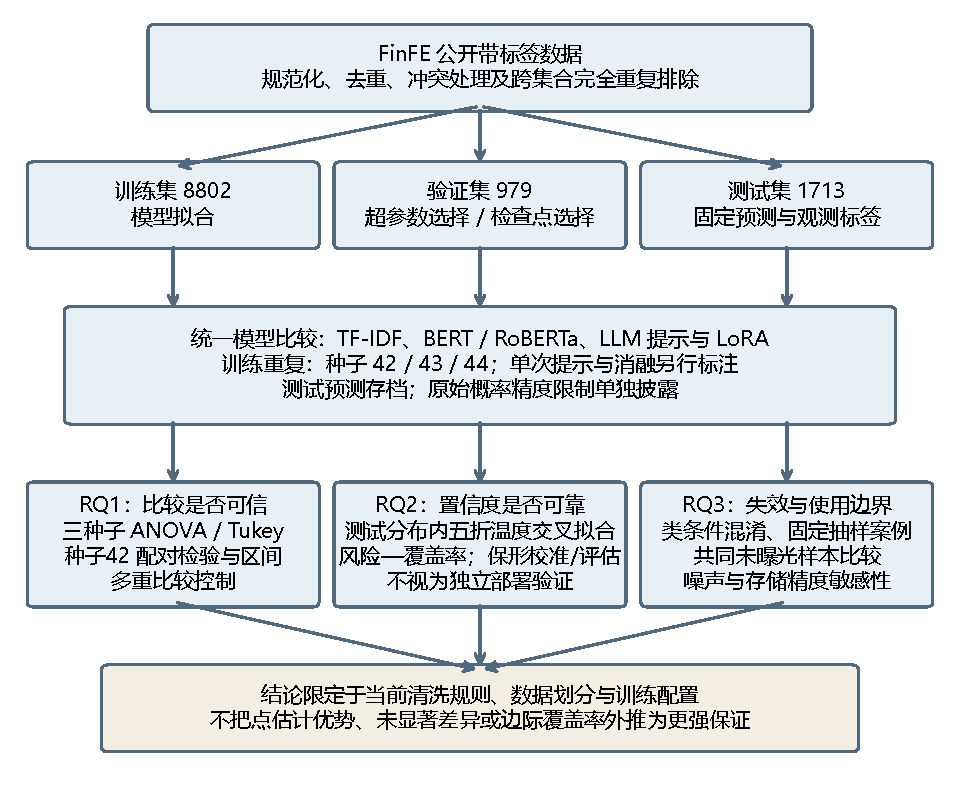
\includegraphics[width=\linewidth,height=0.80\textheight,keepaspectratio]{figures/fig_research_flow.pdf}
\caption{研究流程及数据使用边界}\label{fig:1-1}\end{figure}

图中训练集用于参数拟合，验证集用于超参数或检查点选择。测试集先生成固定预测，之后用于统计比较和描述性错误分析；温度缩放与保形预测则在这批测试记录内部另行分折或划分校准、评估部分。这些内部重用不等于独立外部验证，不能据此宣称得到经部署验证的温度或拒答阈值。

\FloatBarrier\subsection{研究贡献}

本文不提出新的模型结构，而提供当前公开数据版本下的可复核实证证据：

（1）\textbf{数据审计。} 区分训练与验证曝光，在共同未曝光文本上比较清洗策略。

（2）\textbf{条件性比较。} 分别报告训练随机性、测试样本误差及多重比较后的结论。

（3）\textbf{可靠性分解。} 不混同概率校准、选择性准确率和集合覆盖，并披露精度限制。

（4）\textbf{可追溯错误分析。} 报告类指标与固定抽样案例，不将个案解释写成因果结论。

\FloatBarrier\subsection{论文结构}

本文共五章。第 1 章提出研究问题与技术路线；第 2 章比较相关研究并交代评价方法；第 3 章说明数据审计、模型配置与统计设计；第 4 章按照总体性能、差异可信度、概率可靠性和错误边界展开分析；第 5 章总结限定结论，并明确补充验证的条件与优先级。

\clearpage\section{相关研究与评价方法}

本章先梳理与研究问题直接相关的实证与方法工作，再说明本文如何把模型输出转换为可比较的统计证据。重点不是罗列模型原理，而是交代各项方法能够回答什么、不能回答什么。

\FloatBarrier\subsection{相关研究与本文定位}

\subsubsection{从领域适配到中文金融任务}

金融文本中的词语情感依赖领域语境，通用词表可能误解财务术语\cite{ref6}。FinBERT 在 Financial PhraseBank 与 FiQA 等金融任务上研究预训练语言模型的适配\cite{ref8}；Financial PhraseBank 本身也以不同标注一致性水平组织数据\cite{ref20}。这些工作提示：表征能力与标签定义必须一起讨论，不能只比较模型大小。

随着生成式大模型发展，Instruct-FinGPT 将监督情感数据转换为指令数据，关注金融数值与语境理解\cite{ref16}；BBT-Fin 则构建中文金融语料、模型与涵盖理解和生成的评测基准\cite{ref19}。较新的轻量大模型研究已比较 Qwen3-8B 等模型，并包含 Chinese Finance Sentiment 数据\cite{ref18}。因此，中文任务与低资源微调并非空白；本文必须说明相同方法在何种数据版本与评估口径下产生什么证据，而非重复``首次用于中文''的叙述。

\subsubsection{从分类分数到可靠性证据}

单一准确率不能同时说明模型是否稳定、概率是否可信以及何时应该拒答。训练算法比较中的随机性问题已有系统讨论\cite{ref21}；温度缩放关注概率与频率的一致性\cite{ref22}；选择性分类关注风险与覆盖的权衡\cite{ref23}；LoRA 集成研究则从低秩适配的后验近似角度量化不确定性\cite{ref24}。这些是不同问题的解决工具，不能把其中一个指标改善解释为``模型全面可靠''。

\begin{table}[htbp]
\centering
\begin{minipage}{\textwidth}
\setlength{\tabcolsep}{3pt}
\renewcommand{\arraystretch}{1.16}
\setstretch{1.0}\fontsize{10.5}{13.5}\selectfont
\caption{代表性研究的证据侧重点与本文衔接}\label{tab:2-1}
\begin{tabular}{>{\raggedright\arraybackslash}p{\dimexpr 0.200000\linewidth-1.600000\tabcolsep\relax}>{\raggedright\arraybackslash}p{\dimexpr 0.230000\linewidth-1.840000\tabcolsep\relax}>{\raggedright\arraybackslash}p{\dimexpr 0.250000\linewidth-2.000000\tabcolsep\relax}>{\raggedright\arraybackslash}p{\dimexpr 0.320000\linewidth-2.560000\tabcolsep\relax}}
\toprule
\textbf{研究} & \textbf{任务或数据范围} & \textbf{核心侧重点} & \textbf{本文的对应取舍} \\
\midrule
FinBERT\cite{ref8} & Financial PhraseBank、FiQA & 金融领域适配与分类表现 & 将强编码器作为基线；不跨语言、跨划分直接比较分数 \\
BBT-\allowbreak{}Fin\cite{ref19} & 中文金融理解与生成基准 & 语料、模型及统一基准建设 & 审计实际下载的 FinFE 文件，区分论文划分与公开文件 \\
Instruct-\allowbreak{}FinGPT\cite{ref16} & 金融情感任务 & 指令微调、数值及语境理解 & 比较提示与监督微调；用错误案例检查局部语境 \\
轻量 LLM 比较\cite{ref18} & 五个金融数据集，含中文 & 模型、数据量与多场景泛化 & 不将中文 Qwen3 微调视为新方法；重点审计当前比较的可信度 \\
温度缩放\cite{ref22} & 现代神经网络分类 & 事后概率校准 & 使用分折拟合，披露内部评估及概率精度限制 \\
LoRA 集成\cite{ref24} & Mistral-\allowbreak{}7B 与三个多项选择任务 & 低秩适配集成的不确定性 & 本文未复现集成；多种子比较不等同于集成后验推断 \\
\bottomrule\end{tabular}
\par\vspace{3pt}{\fontsize{10}{12.5}\selectfont 注：本表比较研究目标与本文取舍，不是统一排行榜，也不声称未在表中列出的分析在相应论文中不存在。\par}
\end{minipage}
\end{table}

\subsubsection{本文补充的实证证据}

上述研究分别提供了领域适配、任务资源和可靠性方法。本文将它们用于同一批可追溯的预测，形成从数据质量到效应区间、概率校准和失效案例的证据链。其增量是当前 FinFE 公开文件版本下的审计与综合评价，不是新的 LoRA 算法，也不是对已有所有模型的全面复现。下文仅保留理解这一评价设计所需的模型与统计方法。

\FloatBarrier\subsection{文本表示与传统机器学习方法}

\subsubsection{TF-\allowbreak{}IDF 文本表示}

TF-IDF 将字符片段转换为稀疏向量。本文实现使用次线性词频与平滑逆文档频率：对在文档 d 中出现的片段 t，未归一化权重为：

\begin{equation}\operatorname{tfidf}(t,d)=[1+\log\operatorname{tf}(t,d)]\left\{1+\log\frac{1+N}{1+\operatorname{df}(t)}\right\}\tag{2-1}\label{eq:2-1}\end{equation}

其中 tf(t, d) 为出现次数，N 为文档数，df(t) 为包含片段 t 的文档数；未出现片段权重为零，最后对文档向量作 L2 归一化。该式对应实验代码的 sublinear\_tf=True 及默认平滑 IDF，而非不带平滑的简化公式。

本文采用 1～3 元字符 n-gram，不依赖分词。它保留短片段内部顺序，但不显式建模较远上下文，适合作为检验复杂模型增益的低成本基线。

\subsubsection{逻辑回归}

多分类逻辑回归（softmax 回归）假设样本 x 属于第 k 类的概率为：

\begin{equation}P(y=k\mid x)=\frac{\exp(w_k\cdot x+b_k)}{\sum_j\exp(w_j\cdot x+b_j)}\tag{2-2}\label{eq:2-2}\end{equation}

模型参数通过最大化训练数据的对数似然（等价于最小化交叉熵损失）估计，并通常加入 L2 正则项防止过拟合。逻辑回归结构简单、训练快，能直接输出类别概率，是文本分类中常用的基线方法。

\subsubsection{支持向量机}

线性支持向量机（SVM）的思想是在特征空间中寻找一个超平面，使两类样本之间的间隔最大。其优化目标为：

\begin{equation}\min\;\frac12\lVert w\rVert^2+C\sum_i\max\!\left(0,1-y_i(w\cdot x_i+b)\right)\tag{2-3}\label{eq:2-3}\end{equation}

其中 C 控制对误分类的惩罚强度。多分类问题可以通过``一对其余''的方式转化为多个二分类问题。TF-IDF 特征维度高而稀疏，线性 SVM 在这类数据上通常表现良好。

\FloatBarrier\subsection{预训练语言模型}

\subsubsection{Transformer 与自注意力机制}

Transformer\cite{ref25} 是目前主流语言模型的基础结构，其核心是自注意力（self-attention）机制。对于输入序列，每个位置的向量通过三个线性变换分别得到查询 Q、键 K 和值 V，注意力输出为：

\begin{equation}\operatorname{Attention}(Q,K,V)=\operatorname{softmax}\!\left(\frac{QK^{\mathsf T}}{\sqrt{d_k}}\right)V\tag{2-4}\label{eq:2-4}\end{equation}

其中 d\_k 为查询和键的维度。相对于字符片段基线，自注意力提供上下文相关表示；本文不修改注意力结构\cite{ref25}。

\subsubsection{BERT 与 RoBERTa-\allowbreak{}wwm-\allowbreak{}ext}

BERT\cite{ref7} 使用双向编码器及掩码预训练。本文采用标准序列分类微调，在预训练表示上接分类层，并更新全部参数。

在中文场景中，Cui 等\cite{ref9}提出了全词掩码（whole word masking）策略：遮盖时以词为单位，而不是只遮盖单个汉字，使模型更好地学习词级语义。RoBERTa-wwm-ext 在此基础上采用了 RoBERTa 的训练方式，并使用了更大规模的中文语料，是中文文本分类中常用的强基线。本文不把通用中文 RoBERTa 描述为金融领域专用模型。

\FloatBarrier\subsection{大语言模型与参数高效微调}

\subsubsection{大语言模型}

本文选取 Qwen3-8B\cite{ref11}、Qwen2.5-7B-Instruct 和 GLM-4-9B-Chat 三个生成式开源模型，分别比较提示与微调。通用缩放规律\cite{ref26} 不保证特定金融任务上的优势，仍须与监督编码器在相同划分上直接比较。

\subsubsection{零样本与少样本提示}

大模型可以不经训练、直接通过提示词（prompt）完成分类任务。零样本（zero-shot）提示只给出任务说明和待分类文本，例如``判断下面这条股民评论的情感倾向，只回答消极、中性或积极''；少样本（few-shot）提示则在任务说明后附上若干带标签的示例，让模型通过上下文学习（in-context learning）模仿示例作答\cite{ref10}。提示方法不需要训练，但效果依赖提示词的设计，且通常不如有监督微调。

\subsubsection{基于标签词的概率提取}

生成式大模型输出的是文本，而统计评价和校准分析需要每个类别的概率。本文采用标签词概率提取的方法：在提示词末尾让模型生成答案时，读取模型在第一个输出位置上对三个标签词（``消极''\,``中性''\,``积极''）首个词元的 logit 值 z\_k，再做 softmax 归一化：

\begin{equation}p_k=\frac{\exp(z_k)}{\sum_j\exp(z_j)},\quad k\in\{\text{消极},\text{中性},\text{积极}\}\tag{2-5}\label{eq:2-5}\end{equation}

取概率最大的类别作为预测结果，最大概率作为模型的置信度。这种做法保证了输出一定落在三个类别之内，也使大模型可以和 BERT 等模型一样计算校准指标。

\subsubsection{LoRA 低秩适配}

全参数微调需要更新模型的全部参数。以 80 亿参数的模型为例，仅参数、梯度和优化器状态就需要上百 GB 显存，远超单张消费级显卡的容量。参数高效微调方法只训练少量新增参数，其中 LoRA（low-rank adaptation）\cite{ref14} 是最常用的一种。

LoRA 的基本假设是：模型在适应新任务时，权重的变化量是``低秩''的，即可以用两个小矩阵的乘积近似。对于预训练权重 W\(_{0}\) \(\in\) \(\mathbb{R}\)\^{}(d\(\times\)k)，LoRA 冻结 W\(_{0}\)，只训练两个低秩矩阵 B \(\in\) \(\mathbb{R}\)\^{}(d\(\times\)r) 和 A \(\in\) \(\mathbb{R}\)\^{}(r\(\times\)k)：

\begin{equation}h=W_0x+\Delta Wx=W_0x+\frac{\alpha}{r}BAx\tag{2-6}\label{eq:2-6}\end{equation}

其中秩 r 远小于 d 和 k（本文取 4～32），\(\alpha\) 为缩放系数。初始化时 B 为零矩阵，使训练开始时模型与原模型完全相同。本文的主比较保持秩固定，额外消融才改变 r，以免把模型家族差异与秩选择混为一谈。

\subsubsection{QLoRA 量化微调}

QLoRA\cite{ref15} 将冻结的基础权重量化，并训练低秩适配器。本文采用 4-bit NF4、双重量化和 bf16 计算，与非量化配置作单次比较；是否节省资源、分数相差多少由实验报告，不预先假定两者等效。

\FloatBarrier\subsection{分类评价指标}

设测试集中第 k 类的真正例、假正例和假反例个数分别为 TP\_k、FP\_k 和 FN\_k，则该类的精确率、召回率和 F1 值为：

\begin{equation}\begin{aligned}P_k&=\frac{\mathrm{TP}_k}{\mathrm{TP}_k+\mathrm{FP}_k},\quad R_k=\frac{\mathrm{TP}_k}{\mathrm{TP}_k+\mathrm{FN}_k},\\ \mathrm{F1}_k&=\frac{2P_kR_k}{P_k+R_k}\end{aligned}\tag{2-7}\label{eq:2-7}\end{equation}

准确率（accuracy）为预测正确的样本占全部样本的比例。宏平均 F1（Macro-F1）为各类别 F1 的简单平均：

\begin{equation}\text{Macro-F1}=\frac1K\sum_k\mathrm{F1}_k\tag{2-8}\label{eq:2-8}\end{equation}

准确率容易被样本多的类别主导。本文数据中积极类约占一半，若模型偏向预测积极，准确率仍可能较高，而宏平均 F1 对每个类别一视同仁，更能反映模型在少数类上的表现，因此本文以宏平均 F1 为主要指标。

\FloatBarrier\subsection{模型比较的统计检验}

模型分数之间的差异可能来自两种随机性：一是\textbf{训练随机性}，即同一模型换一个随机种子重新训练，分数也会波动；二是\textbf{测试样本抽样误差}，即测试集只是所有可能样本中的一个有限样本，换一批测试样本，分数也会不同\cite{ref21}。本文针对这两种来源分别使用不同的检验方法。

\subsubsection{方差分析与多重比较}

针对训练随机性，本文对 BERT、RoBERTa 和三个 LoRA 大模型分别用 r 个不同随机种子各训练一次，把每次的宏平均 F1 看作一个观测值，用单因素方差分析（ANOVA）检验各模型的平均分数是否相同。其检验统计量为：

\begin{equation}F=\frac{\sum_i n_i(\bar y_i-\bar y)^2/(g-1)}{\sum_i\sum_j(y_{ij}-\bar y_i)^2/(N-g)}\tag{2-9}\label{eq:2-9}\end{equation}

其中 g 为模型个数，\(\bar y\)\_i 为第 i 个模型的平均分数，\(\bar y\) 为总平均。F 值越大，说明模型间差异相对于种子间波动越大。当各组方差可能不等时，可使用 Welch 方差分析作为稳健性检验。若方差分析显著，再用 Tukey HSD 检验进行两两比较，它在所有两两比较中同时控制第一类错误率。

\subsubsection{McNemar 检验}

针对测试样本抽样误差，McNemar 检验\cite{ref27} 用于比较两个模型在同一测试集上的准确率。设 b 为模型甲正确而模型乙错误的样本数，c 为模型甲错误而模型乙正确的样本数，在``两模型准确率相同''的原假设下，b 应服从参数为 (b + c, 0.5) 的二项分布；样本较多时，也可用统计量：

\begin{equation}\chi^2=\frac{(\lvert b-c\rvert-1)^2}{b+c}\tag{2-10}\label{eq:2-10}\end{equation}

近似服从自由度为 1 的卡方分布。该检验只利用两个模型预测不一致的样本，考虑了两模型在同一批样本上的配对关系，是比较分类器的常用方法\cite{ref21}。

\subsubsection{配对 Bootstrap 置信区间}

宏平均 F1 不是简单的比例，难以写出其差值的解析分布。Bootstrap 方法\cite{ref28} 通过重抽样来近似统计量的抽样分布：从 n 个测试样本中有放回地抽取 n 个，组成一个新的测试集，在其上计算两个模型的 F1 差值；重复 B 次，取差值的 2.5\% 和 97.5\% 分位数作为单个比较的 95\% 百分位区间。``配对''指两个模型每次都在同一批重抽样样本上计算，从而保留两者的相关性。本文对模型间差值采用 B = 50000，固定重抽样种子为 20261012；将五个主要比较模型的全部十对构成一个比较家族，另报告 Bonferroni 调整后的 0.25\% 和 99.75\% 分位数区间，以获得名义 95\% 的家族同时覆盖率。该区间仍依赖 Bootstrap 近似，单个未调整区间不跨 0 不能直接解释为多重比较后的显著结果。单模型、单次运行的区间仍使用 B = 2000，两种口径分别标注。

\subsubsection{Holm 多重比较校正}

同时进行 m 次检验时，即使每次检验的显著性水平都是 0.05，至少出现一次误判的概率也会明显增大。Holm 方法\cite{ref29} 将 m 个 p 值从小到大排序为 p\(_{(1)}\) \(\le\) \ldots{} \(\le\) p\(_{(m)}\)，依次将 p\(_{(i)}\) 与 \(\alpha\)/(m \(-\) i + 1) 比较，一旦某个 p 值不满足条件，就停止并不再拒绝其后原假设。等价地，校正后的 p 值为：

\begin{equation}\tilde p_{(i)}=\max_{j\le i}\min\{1,(m-j+1)p_{(j)}\}\tag{2-11}\label{eq:2-11}\end{equation}

Holm 方法在控制总体第一类错误率的同时，比 Bonferroni 校正更不保守。

\FloatBarrier\subsection{置信度校准}

\subsubsection{校准的含义与度量}

如果一个模型对一批样本给出的置信度都是 80\%，那么这批样本中应当约 80\% 被预测正确，这样的模型称为``校准良好''的模型。研究发现，现代深度神经网络往往过度自信，即置信度系统性地高于实际准确率\cite{ref22}；LoRA 微调的大模型也存在类似问题\cite{ref24}。

期望校准误差（expected calibration error, ECE）是最常用的校准度量。将样本按置信度划分为 M 个区间（本文取 M = 15），第 m 个区间的样本集合为 B\_m，则：

\begin{equation}\mathrm{ECE}=\sum_m\frac{\lvert B_m\rvert}{n}\,\bigl\lvert\operatorname{acc}(B_m)-\operatorname{conf}(B_m)\bigr\rvert\tag{2-12}\label{eq:2-12}\end{equation}

其中 acc(B\_m) 和 conf(B\_m) 分别为该区间内的实际准确率和平均置信度。ECE 越小，校准越好。以横轴为置信度、纵轴为准确率画出的图称为可靠性图，完全校准的模型应落在对角线上。

\subsubsection{温度缩放}

温度缩放（temperature scaling）\cite{ref22} 是一种简单有效的校准方法：用一个标量 T \textgreater{} 0 除以模型输出的 logit，再做 softmax：

\begin{equation}p_k=\frac{\exp(z_k/T)}{\sum_j\exp(z_j/T)}\tag{2-13}\label{eq:2-13}\end{equation}

T \textgreater{} 1 会使概率分布更``平''，降低过高的置信度；T \textless{} 1 则相反。T 通常在一组留出样本上通过最小化负对数似然确定（本文的具体做法见 3.7.3 节，采用测试集上的 5 折交叉拟合）。由于除以同一个正数不改变 logit 的大小顺序，温度缩放不会改变预测类别和准确率，只调整置信度。

\FloatBarrier\subsection{选择性预测}

在实际应用中，模型可以对没把握的样本``拒绝回答''，交给人工处理，这称为选择性预测（selective prediction）\cite{ref23,ref30}。具体做法是设定置信度阈值 \(\tau\)，只对置信度不低于 \(\tau\) 的样本给出预测。被模型回答的样本占全部样本的比例称为\textbf{覆盖率}，在这些样本上的错误率称为\textbf{风险}。

阈值越高，覆盖率越低，但被回答样本的准确率通常越高。将阈值从高到低变化，可以得到风险---覆盖率曲线，曲线下面积 AURC（area under the risk-coverage curve）综合反映了模型的置信度排序能力：AURC 越小，说明模型越能把错误样本排在低置信度的位置。与 ECE 关注``置信度的数值是否准确''不同，AURC 关注``置信度的高低顺序是否合理''。

\FloatBarrier\subsection{保形预测}

选择性预测只能给出``回答或不回答''，保形预测（conformal prediction）\cite{ref31,ref32} 则给出一个类别集合，并提供有限样本下的覆盖率保证。以分割保形预测为例：取一组未参与训练的校准样本，计算每个样本的非一致性分数 s\_i = 1 \(-\) p(y\_i \textbar{} x\_i)，即模型给真实类别的概率越低，分数越高；取分数的修正分位数

\begin{equation}\hat q=s\text{ 的第 }\lceil(n+1)(1-\alpha)\rceil\text{ 个次序统计量}\tag{2-14}\label{eq:2-14}\end{equation}

对新样本输出集合 C(x) = \{k : 1 \(-\) p\_k(x) \(\le\) \(\hat q\)\}。只要校准样本与新样本是可交换的（如独立同分布），就有

\begin{equation}P\bigl(y\in C(x)\bigr)\ge 1-\alpha\tag{2-15}\label{eq:2-15}\end{equation}

这一保证不依赖于模型是否校准良好，也不需要指定某个参数分布族，但仍要求校准样本与新样本的交换性，并保持预测模型和评分规则固定。它是对校准集与新样本随机性取平均后的边际保证，不保证每次固定划分的经验覆盖率都达到目标。平均集合大小反映预测集合的效率，但不能单独代替对子群覆盖和适应性的评估。

需要注意的是，式（2-15）只保证整体（边际）覆盖率，某些困难类别的覆盖率可能低于 1 \(-\) \(\alpha\)；筛选出的单元素集合也不会自动获得同样的条件正确率保证。Mondrian 保形预测\cite{ref31} 对每一类别分别计算 \(\hat q\)，在相应类内交换性条件下给出类别条件覆盖保证，但这仍不同于``单元素答案正确率''的保证。

\FloatBarrier\subsection{标注一致性与标签噪声}

有监督学习使用观测标签作为学习目标，但标签之间可能存在分歧。对固定两名标注者，Cohen \(\kappa\) 可写为：

\begin{equation}\kappa=\frac{p_o-p_e}{1-p_e}\tag{2-16}\label{eq:2-16}\end{equation}

其中 p\_o 为观察一致率，p\_e 为两名标注者类别边际比例乘积之和。本文没有固定标注者身份，重复也未必来自独立复标，故只定义描述性的 K\_pair = (p\_o \(-\) p\_e,pair)/(1 \(-\) p\_e,pair)，其中 p\_e,pair = \(\Sigma\)\_c \(\pi\)\_c\(^{2}\)，\(\pi\)\_c 为配对两端汇总类别比例。它与一致率采用同一配对加权口径，不解释标注者可靠性，也不称为标准 Cohen \(\kappa\)。

进一步，假设给定真实类别后，两次标注相互独立、均以相同概率 q 标对，标错时等可能地选择其余两类，则 p\_o = q\(^{2}\) + (1 \(-\) q)\(^{2}\)/2。取 q \(\ge\) 1/3 的分支可得：

\begin{equation}q=\frac{1+\sqrt{6p_o-2}}{3}\tag{2-17}\label{eq:2-17}\end{equation}

q 仅在上述独立、同质、对称噪声假设下有意义。缺少独立复标与金标准、重复文本非随机、清洗改变样本构成，均使它不能被解释为测试集实测上限或人工水平。

\FloatBarrier\subsection{本章小结}

本章把领域适配研究与统计评价问题衔接起来：模型提供分类与概率输出，多种子和配对分析分别考察不同不确定性，校准、选择性预测与保形预测回答不同可靠性问题。本文使用这些已有方法构造可复核评价，不将它们作为新算法；第 3 章给出具体实施口径。

\clearpage\section{数据与研究方法}

\FloatBarrier\subsection{数据来源}

本文使用的数据集为 FinFE（Financial Forum Emotion），它是中文金融评测基准 BBT-CFLEB 中的情感分类子任务\cite{ref19}。FinFE 的文本来自金融社交媒体上的股民评论，每条评论被标注为消极、中性、积极三类情感之一。与新闻标题、研报等规范文本相比，股民评论篇幅短、口语化程度高，常夹杂股票代码、网络用语和反讽表达，对模型的语义理解能力要求较高。

原论文描述的数据划分为训练集 8000 条、验证集 1000 条、测试集 1000 条，但项目公开仓库中实际提供的文件与之不同：train\_list.json 含 16157 条带标签样本，eval\_list.json 含 2020 条带标签样本，problem\_list.json 含 2020 条无标签样本（排行榜测试集，标签未公开）。由于无标签样本无法用于评估，本文仅使用前两个文件，并以公开文件的实际内容为准重新构建数据集。

\FloatBarrier\subsection{数据质量检查与清洗}

在正式实验前，本文对原始数据进行了质量检查，发现三类问题：

\begin{enumerate}
\def\labelenumi{\arabic{enumi}.}
\tightlist
\item
  训练文件中存在大量重复文本，其中 773 条文本在不同位置被标注为不同标签（标签冲突）；
\item
  原始 eval\_list 的 2020 条记录中，有 1097 条规范化文本也出现在原始训练文件中。原始训练文件随后还会划出验证集，因此这首先说明开发数据与评估数据存在重叠，实际训练曝光与验证曝光需另行区分；
\item
  在分别完成文件内去重、去冲突后，两文件仍有 1092 个重叠文本，其中 228 个跨文件标签不同，说明部分记录的标签存在分歧。
\end{enumerate}

针对这些问题，本文制定了如下清洗规则，并固定随机种子为 42，保证结果可复现：

\begin{enumerate}
\def\labelenumi{\arabic{enumi}.}
\tightlist
\item
  对文本做 Unicode NFKC 规范化，并去除首尾空白字符；
\item
  同一文件内的重复文本，若标签一致则只保留一条，若标签冲突则整组删除；
\item
  以 eval\_list 作为测试集来源，删除其中与训练文件标签不一致的 228 条样本；
\item
  从训练池中删除与文件内清洗后的评估集合重叠的全部文本，包括随后从测试集剔除的 228 个跨文件冲突文本，排除规范化后完全相同文本的跨集合重叠；
\item
  对剩余训练数据按类别分层抽样，划出 10\% 作为验证集，用于超参数选择和早停。
\end{enumerate}

清洗过程各步骤的样本数量变化见表~\ref{tab:3-1}。

\begin{table}[htbp]
\centering
\begin{minipage}{\textwidth}
\setlength{\tabcolsep}{3pt}
\renewcommand{\arraystretch}{1.16}
\setstretch{1.0}\fontsize{10.5}{13.5}\selectfont
\caption{数据清洗过程}\label{tab:3-1}
\begin{tabular}{>{\raggedright\arraybackslash}p{\dimexpr 0.780000\linewidth-3.120000\tabcolsep\relax}>{\raggedright\arraybackslash}p{\dimexpr 0.220000\linewidth-0.880000\tabcolsep\relax}}
\toprule
\textbf{步骤} & \textbf{数量} \\
\midrule
原始训练文件 train\_\allowbreak{}list & 16157 \\
原始评估文件 eval\_\allowbreak{}list & 2020 \\
训练文件：删除重复样本（标签一致） & 3725 \\
训练文件：删除标签冲突的文本 & 773 \\
评估文件：删除重复样本（标签一致） & 61 \\
评估文件：删除标签冲突的文本 & 9 \\
评估文件中与训练文件重复但标签不同的文本（从测试集删除） & 228 \\
训练文件内清洗后与评估集合重叠的文本（含 228 个跨文件冲突文本，均删除） & 1092 \\
\bottomrule\end{tabular}
\end{minipage}
\end{table}

清洗后最终得到训练集 8802 条、验证集 979 条、测试集 1713 条，各数据集的类别分布见表~\ref{tab:3-2} 和图~\ref{fig:3-1}。

\begin{table}[htbp]
\centering
\begin{minipage}{\textwidth}
\setlength{\tabcolsep}{3pt}
\renewcommand{\arraystretch}{1.16}
\setstretch{1.0}\fontsize{10.5}{13.5}\selectfont
\caption{清洗后各数据集类别分布}\label{tab:3-2}
\begin{tabular}{>{\raggedright\arraybackslash}p{\dimexpr 0.200000\linewidth-2.000000\tabcolsep\relax}>{\raggedright\arraybackslash}p{\dimexpr 0.200000\linewidth-2.000000\tabcolsep\relax}>{\raggedright\arraybackslash}p{\dimexpr 0.200000\linewidth-2.000000\tabcolsep\relax}>{\raggedright\arraybackslash}p{\dimexpr 0.200000\linewidth-2.000000\tabcolsep\relax}>{\raggedright\arraybackslash}p{\dimexpr 0.200000\linewidth-2.000000\tabcolsep\relax}}
\toprule
\textbf{数据集} & \textbf{消极} & \textbf{中性} & \textbf{积极} & \textbf{合计} \\
\midrule
训练集 & 2044（23.2\%） & 1845（21.0\%） & 4913（55.8\%） & 8802 \\
验证集 & 227（23.2\%） & 205（20.9\%） & 547（55.9\%） & 979 \\
测试集 & 461（26.9\%） & 438（25.6\%） & 814（47.5\%） & 1713 \\
\bottomrule\end{tabular}
\end{minipage}
\end{table}

\begin{figure}[htbp]\centering
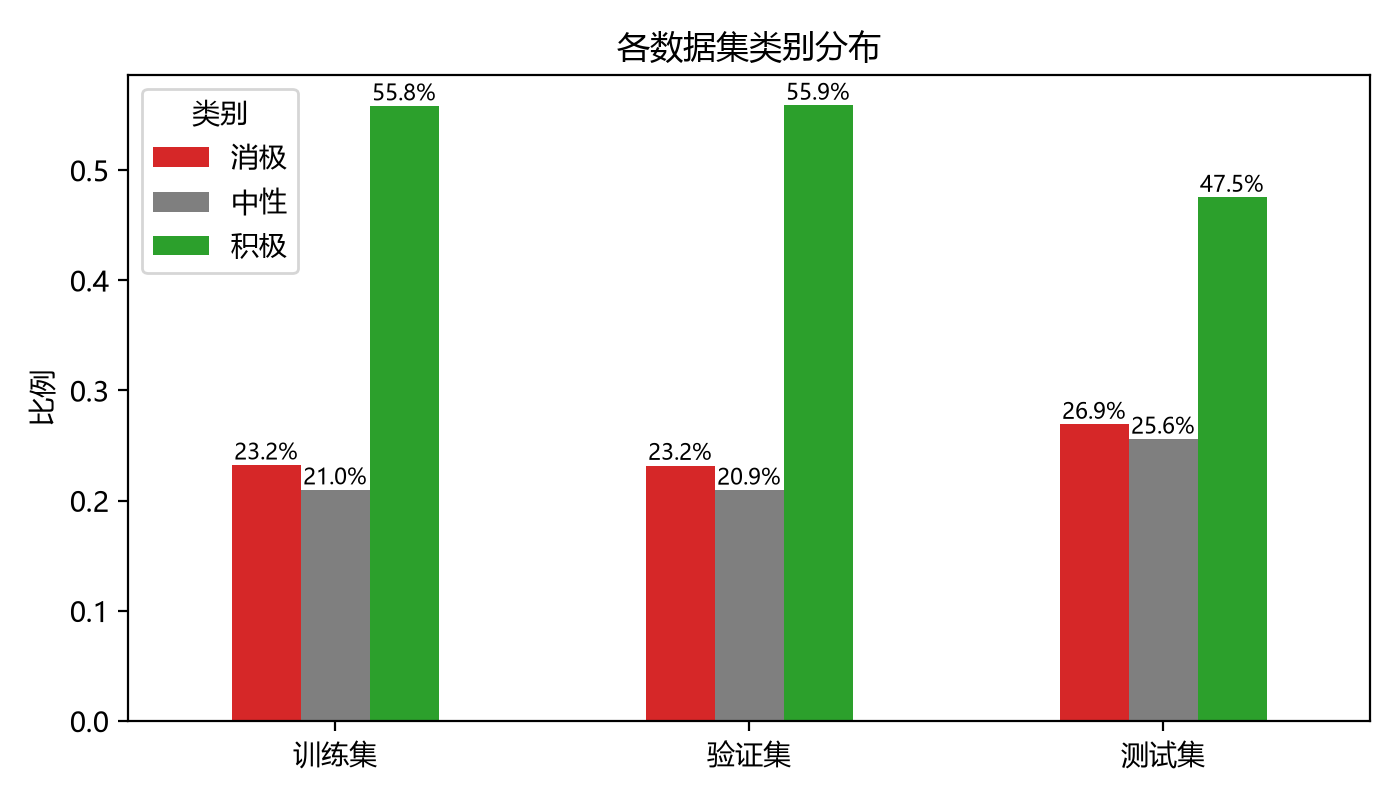
\includegraphics[width=\linewidth,height=0.80\textheight,keepaspectratio]{figures/fig_label_dist.png}
\caption{各数据集类别分布}\label{fig:3-1}\end{figure}

对``数据集 \(\times\) 类别''列联表做卡方检验，得到 \(\chi^{2}\) = 41.09，自由度为 4，p = 2.6\(\times\)10\(^{-8}\)，说明测试集的类别比例与训练集存在显著差异：测试集中积极类占比较低，消极类和中性类占比较高。该差异与去重、冲突删除及重新划分后的样本构成有关，不能单独归因于去除泄露。由于类别分布不均衡，且训练集与测试集分布不完全一致，本文以宏平均 F1 值（Macro-F1）作为主要评价指标，准确率作为辅助指标。依据跨文件标签一致性删除评估记录会改变评估对象，可能排除更难或更有歧义的样本；因此后续结论限于该清洗规则下的数据，不能视为对原始评论总体的无偏估计。本文也未系统排除近重复和预训练数据污染。

\FloatBarrier\subsection{描述性统计分析}

\subsubsection{文本长度}

FinFE 文本整体很短，各类别的长度统计见表~\ref{tab:3-3}。积极类评论平均长度为 22.6 个字符，明显长于消极类（19.6）和中性类（19.7）。由于长度分布明显右偏（见图~\ref{fig:3-2}），本文采用非参数的 Kruskal-Wallis 检验比较三类文本的长度分布，结果为 H = 157.21，p = 7.3\(\times\)10\(^{-35}\)，差异极显著。这说明文本长度本身携带一定的情感信息，但三类之间的长度分布重叠很大，仅靠长度无法有效区分情感。

\begin{table}[htbp]
\centering
\begin{minipage}{\textwidth}
\setlength{\tabcolsep}{3pt}
\renewcommand{\arraystretch}{1.16}
\setstretch{1.0}\fontsize{10.5}{13.5}\selectfont
\caption{各类别文本长度（字符）}\label{tab:3-3}
\begin{tabular}{>{\raggedright\arraybackslash}p{\dimexpr 0.142857\linewidth-2.000000\tabcolsep\relax}>{\raggedright\arraybackslash}p{\dimexpr 0.142857\linewidth-2.000000\tabcolsep\relax}>{\raggedright\arraybackslash}p{\dimexpr 0.142857\linewidth-2.000000\tabcolsep\relax}>{\raggedright\arraybackslash}p{\dimexpr 0.142857\linewidth-2.000000\tabcolsep\relax}>{\raggedright\arraybackslash}p{\dimexpr 0.142857\linewidth-2.000000\tabcolsep\relax}>{\raggedright\arraybackslash}p{\dimexpr 0.142857\linewidth-2.000000\tabcolsep\relax}>{\raggedright\arraybackslash}p{\dimexpr 0.142857\linewidth-2.000000\tabcolsep\relax}}
\toprule
\textbf{类别} & \textbf{样本数} & \textbf{均值} & \textbf{标准差} & \textbf{最小值} & \textbf{中位数} & \textbf{最大值} \\
\midrule
消极 & 2732 & 19.62 & 13.57 & 4 & 16 & 66 \\
中性 & 2488 & 19.72 & 13.64 & 4 & 16 & 67 \\
积极 & 6274 & 22.56 & 14.26 & 4 & 19 & 68 \\
\bottomrule\end{tabular}
\end{minipage}
\end{table}

\begin{figure}[htbp]\centering
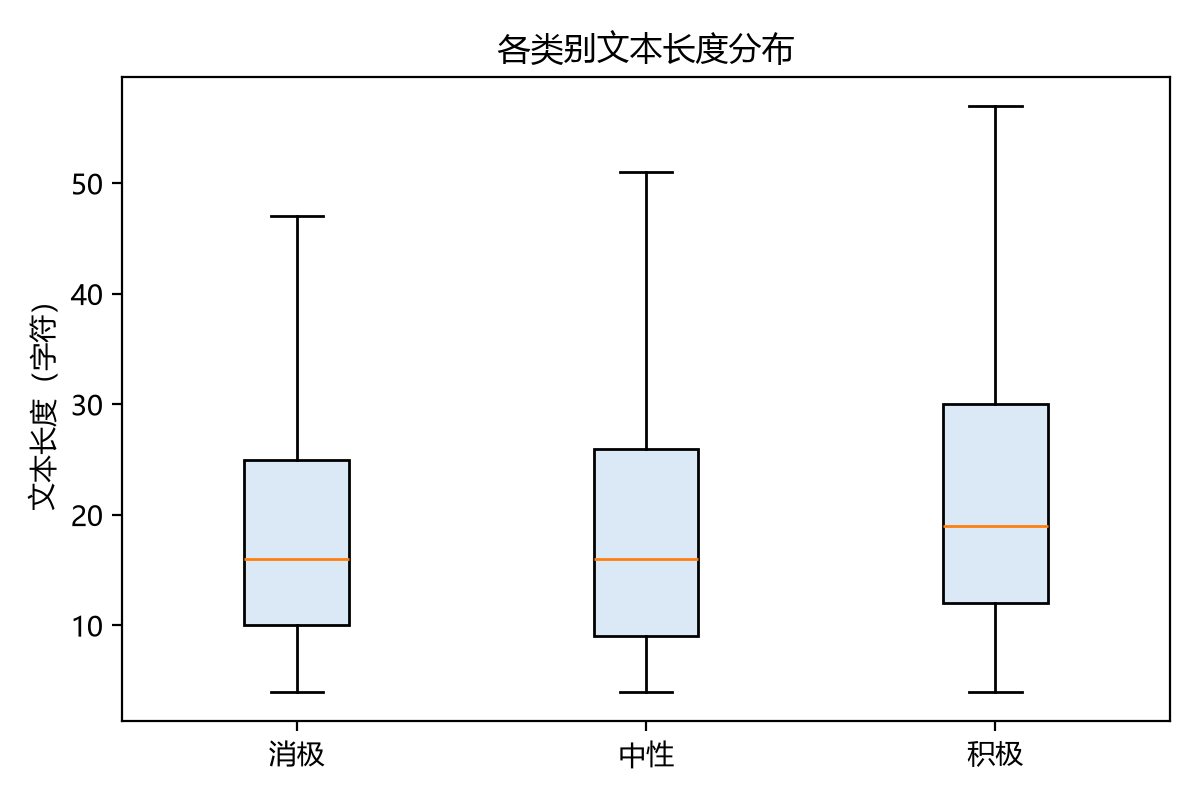
\includegraphics[width=\linewidth,height=0.80\textheight,keepaspectratio]{figures/fig_length_by_label.png}
\caption{各类别文本长度分布}\label{fig:3-2}\end{figure}

\subsubsection{文本特征}

本文进一步统计了否定词、数字、问号和感叹号四类表层特征在各类别中的出现比例，并对每个特征做卡方独立性检验，结果见表~\ref{tab:3-4}。四个特征与情感类别均显著相关（p 均小于 10\(^{-23}\)）：消极类评论更常出现否定词（40.2\%），中性类评论更常出现问号（17.8\%，多为向其他股民提问），积极类评论更常出现感叹号（20.9\%）和数字。中性类的问句特征提示，这一类别中有相当部分评论并不表达明确态度，这可能是后文各模型在中性类上表现最差的原因之一。

\begin{table}[htbp]
\centering
\begin{minipage}{\textwidth}
\setlength{\tabcolsep}{3pt}
\renewcommand{\arraystretch}{1.16}
\setstretch{1.0}\fontsize{10.5}{13.5}\selectfont
\caption{文本特征在各类别中的占比}\label{tab:3-4}
\begin{tabular}{>{\raggedright\arraybackslash}p{\dimexpr 0.166667\linewidth-2.000000\tabcolsep\relax}>{\raggedright\arraybackslash}p{\dimexpr 0.166667\linewidth-2.000000\tabcolsep\relax}>{\raggedright\arraybackslash}p{\dimexpr 0.166667\linewidth-2.000000\tabcolsep\relax}>{\raggedright\arraybackslash}p{\dimexpr 0.166667\linewidth-2.000000\tabcolsep\relax}>{\raggedright\arraybackslash}p{\dimexpr 0.166667\linewidth-2.000000\tabcolsep\relax}>{\raggedright\arraybackslash}p{\dimexpr 0.166667\linewidth-2.000000\tabcolsep\relax}}
\toprule
\textbf{特征} & \textbf{消极} & \textbf{中性} & \textbf{积极} & \textbf{$\chi^{2}$} & \textbf{p} \\
\midrule
含否定词 & 40.2\% & 33.3\% & 29.1\% & 107.352 & 4.9$\times$10$^{-24}$ \\
含数字 & 19.8\% & 27.7\% & 30.5\% & 108.565 & 2.7$\times$10$^{-24}$ \\
含问号 & 8.8\% & 17.8\% & 4.5\% & 408.784 & 1.7$\times$10$^{-89}$ \\
含感叹号 & 15.4\% & 10.8\% & 20.9\% & 135.512 & 3.7$\times$10$^{-30}$ \\
\bottomrule\end{tabular}
\end{minipage}
\end{table}

\subsubsection{高频词}

使用 jieba 分词并去除停用词后，训练集各类别的高频词见图~\ref{fig:3-3}。消极类的高频词包括``垃圾''\,``下跌''\,``跌停''\,``大跌''\,``出货''\,``退市''，积极类包括``涨停''\,``加油''\,``加仓''\,``买入''\,``看好''\,``龙头''，均符合股民的表达习惯。中性类的高频词如``看看''\,``一下''\,``多少''\,``可能''，大多不带情感倾向，进一步印证了中性类以提问和陈述为主的特点。

\begin{figure}[htbp]\centering
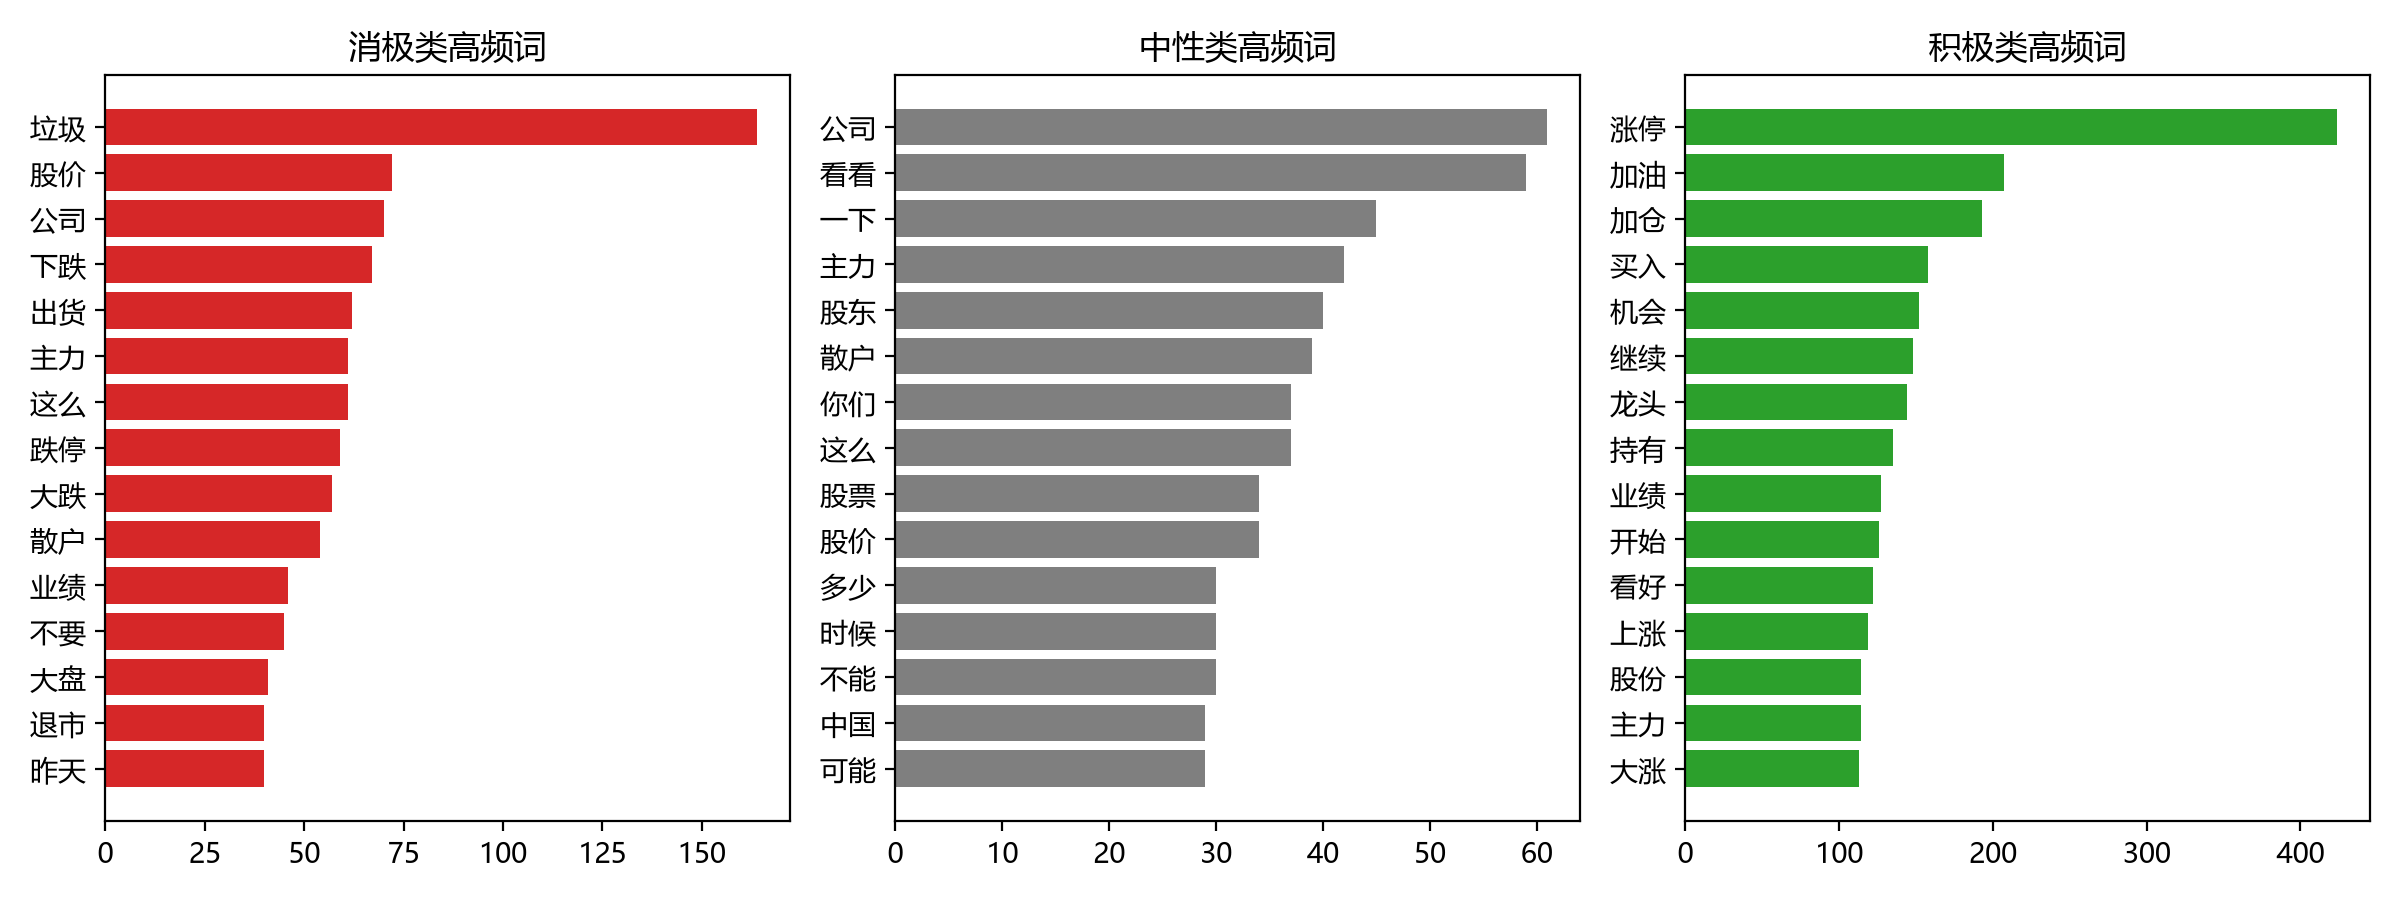
\includegraphics[width=\linewidth,height=0.80\textheight,keepaspectratio]{figures/fig_top_words.png}
\caption{训练集各类别高频词}\label{fig:3-3}\end{figure}

\FloatBarrier\subsection{对比模型}

为全面评估大语言模型的效果，本文设置了四类模型，见表~\ref{tab:3-5}。

\begin{table}[htbp]
\centering
\begin{minipage}{\textwidth}
\setlength{\tabcolsep}{3pt}
\renewcommand{\arraystretch}{1.16}
\setstretch{1.0}\fontsize{10.5}{13.5}\selectfont
\caption{实验模型}\label{tab:3-5}
\begin{tabular}{>{\raggedright\arraybackslash}p{\dimexpr 0.190000\linewidth-1.520000\tabcolsep\relax}>{\raggedright\arraybackslash}p{\dimexpr 0.400000\linewidth-3.200000\tabcolsep\relax}>{\raggedright\arraybackslash}p{\dimexpr 0.130000\linewidth-1.040000\tabcolsep\relax}>{\raggedright\arraybackslash}p{\dimexpr 0.280000\linewidth-2.240000\tabcolsep\relax}}
\toprule
\textbf{类别} & \textbf{模型} & \textbf{参数量} & \textbf{使用方式} \\
\midrule
传统机器学习 & TF-\allowbreak{}IDF + 逻辑回归 /\allowbreak{} 线性 SVM & — & 有监督训练 \\
预训练语言模型 & BERT-\allowbreak{}base-\allowbreak{}Chinese\cite{ref7} & 1.0 亿 & 全参数微调 \\
预训练语言模型 & Chinese-\allowbreak{}RoBERTa-\allowbreak{}wwm-\allowbreak{}ext\cite{ref9} & 1.0 亿 & 全参数微调 \\
大语言模型 & Qwen3-\allowbreak{}8B、Qwen2.5-\allowbreak{}7B-\allowbreak{}Instruct、GLM-\allowbreak{}4-\allowbreak{}9B-\allowbreak{}Chat & 70 亿～94 亿 & 零样本、少样本提示；LoRA 微调 \\
\bottomrule\end{tabular}
\end{minipage}
\end{table}

传统基线采用字符级 1～3 元组的 TF-IDF 特征，分类器的正则化系数 C 在验证集上从 \{0.1, 0.3, 1, 3, 10, 30, 100\} 中选择。线性 SVM 本身不输出概率，本文用 sigmoid 校准（5 折交叉验证）得到三类概率，以便与其他模型统一做校准分析。

预训练语言模型采用标准的序列分类微调：学习率 2\(\times\)10\(^{-5}\)，批大小 32，最多训练 5 轮，前 10\% 步数线性预热后线性衰减，最大序列长度 96，以验证集 Macro-F1 早停（连续 2 轮不提升即停止）。

\FloatBarrier\subsection{大语言模型的分类方法}

\subsubsection{提示设计}

本文将情感分类表述为对话任务。系统提示为``你是一名金融文本情感分析助手。''，用户提示为：

\begin{quote}\small 请判断下面这条股民评论的情感倾向，只能回答“消极”“中性”“积极”三者之一，不要输出其他内容。\par 评论：\{评论文本\}\end{quote}

提示经各模型自带的对话模板渲染后输入模型。对于 Qwen3-8B，本文关闭了其``思考模式''，使模型直接给出答案。少样本设置下，从训练集中每类随机抽取 k 条样本（k = 1 或 3，随机种子 42），以``用户提问---助手回答''的多轮对话形式放在待测评论之前。

\subsubsection{基于标签词的概率提取}

采用第 2 章式（2-5）的标签词方法：读取答案首位置对``消极''\,``中性''\,``积极''三个标签首 token 的 logit，再在这三个值间归一化。代码断言三个 token ID 互异，预测取最大概率类别。它避免了自由生成后的文本解析，但所得概率依赖提示与标签词，并非完整答案字符串的生成概率。

\subsubsection{LoRA 微调}

本文采用第 2 章式（2-6）的 LoRA 结构。本文在注意力层的 q、k、v、o 投影和前馈层的 gate、up、down 投影上都加入 LoRA 模块，主实验取 r = 16、\(\alpha\) = 32、dropout = 0.05。以 Qwen3-8B 为例，可训练参数为 4365 万，仅占总参数量（82.3 亿）的 0.53\%。

训练时在答案的第一个位置上，对正确标签词首 token 计算全词表交叉熵，而不是对完整标签词序列逐 token 计算损失。推理时再将三个标签首 token 的 logits 归一化为三分类概率，两者共享标签映射，但训练损失的分母是全词表。优化器为 AdamW，学习率 1\(\times\)10\(^{-4}\)，有效批大小 16，训练 2 轮，前 5\% 步数线性预热后线性衰减，梯度裁剪阈值 1.0，采用 bf16 混合精度和梯度检查点以节省显存。每轮结束后在验证集上计算 Macro-F1，保留最优一轮的 LoRA 权重用于测试。

为考察量化对效果的影响，本文还实现了 QLoRA\cite{ref15}：以 4-bit NF4 格式加载冻结的基础模型权重（采用双重量化），计算 dtype 设为 bf16；不将适配器各张量精度与量化基础权重的存储精度混为一谈。

\FloatBarrier\subsection{实验环境与重复设计}

全部实验在一台配备 NVIDIA RTX 3090（24 GB 显存）、32 GB 内存的 Windows 计算机上完成，软件环境为 Python 3.11、PyTorch 2.7.1（CUDA 12.8）、transformers、peft 和 bitsandbytes。

为区分模型差异与训练随机性，BERT、RoBERTa 和三个大模型的 LoRA 微调均使用 3 个随机种子（42、43、44）重复训练。零样本推理是确定性的，只运行一次；少样本和消融实验受计算资源限制，只使用种子 42。

\begin{table}[htbp]
\centering
\begin{minipage}{\textwidth}
\setlength{\tabcolsep}{3pt}
\renewcommand{\arraystretch}{1.16}
\setstretch{1.0}\fontsize{10.5}{13.5}\selectfont
\caption{关键实验配置与核验依据}\label{tab:3-6}
\begin{tabular}{>{\raggedright\arraybackslash}p{\dimexpr 0.190000\linewidth-1.140000\tabcolsep\relax}>{\raggedright\arraybackslash}p{\dimexpr 0.650000\linewidth-3.900000\tabcolsep\relax}>{\raggedright\arraybackslash}p{\dimexpr 0.160000\linewidth-0.960000\tabcolsep\relax}}
\toprule
\textbf{对象} & \textbf{关键设置} & \textbf{核验依据} \\
\midrule
TF-\allowbreak{}IDF 特征 & 字符 1～3 元组；min\_\allowbreak{}df=2；次线性词频、平滑 IDF、L2 归一化 & 实现 I \\
LR /\allowbreak{} SVM & C 候选为 0.1、0.3、1、3、10、30、100；实际选择分别为 10、0.3；类别权重 balanced & 记录 R、实现 I \\
SVM 概率 & 训练数据内 5 折 sigmoid 校准；外部验证集选择 C & 实现 I \\
BERT /\allowbreak{} RoBERTa & 学习率 2$\times$10$^{-5}$；批大小 32；长度上限 96；AdamW 权重衰减 0.01 & 记录 R、实现 I \\
BERT /\allowbreak{} RoBERTa 选择 & 最多 5 轮；预热 10\%；验证 F1 连续 2 轮不提升停止；保留验证最优权重 & 实现 I；实际轮数见注 \\
LoRA 主配置 & r=16，$\alpha$=32，dropout=0.05；q/\allowbreak{}k/\allowbreak{}v/\allowbreak{}o 与 gate/\allowbreak{}up/\allowbreak{}down 七类投影 & 记录 R、实现 I \\
LoRA 优化与选择 & 学习率 1$\times$10$^{-4}$；有效批大小 16；训练 2 轮；AdamW 权重衰减 0；预热 5\%；验证最优轮 & 记录 R、实现 I \\
LLM 输入与损失 & 按模型对话模板、左侧填充；当前代码不主动截断；答案首位置全词表交叉熵；推理在三个标签 token 间归一化 & 实现 I \\
重复与单次实验 & BERT、RoBERTa、三个 LoRA：42 /\allowbreak{} 43 /\allowbreak{} 44；提示与配置消融另按单次口径报告 & 记录 R \\
\bottomrule\end{tabular}
\par\vspace{3pt}{\fontsize{10}{12.5}\selectfont 注：R 指 outputs/\allowbreak{}metrics 中实际运行记录，I 指 src/\allowbreak{}baselines 与 src/\allowbreak{}llm 中当前实现；记录与实现共同核对，不把代码默认值冒称为完整历史参数快照。两类编码器在种子 42、43、44 下实际均运行 4、5、4 轮（不是最佳轮次）。LoRA 记录确认主实验未启用 4-\allowbreak{}bit；4-\allowbreak{}bit 是独立消融。微批量未在历史 metrics 中完整保存，故不补写为已证实的运行参数。\par}
\end{minipage}
\end{table}

\FloatBarrier\subsection{评价指标与统计方法}

\subsubsection{分类指标}

按第 2 章式（2-7）和式（2-8）计算类精确率、召回率、F1 与 Macro-F1，准确率为辅助指标。主结果表区分多种子均值与单次区间，错误分析另行报告种子 42 的混淆矩阵，避免把两种口径混用。

\subsubsection{显著性检验}

\textbf{McNemar 与 Holm 校正。} 使用第 2 章式（2-10）的连续性校正检验；不一致样本总数小于 25 时使用精确二项检验。固定 TF-IDF+LR、RoBERTa 与三个 LoRA 模型构成比较集合，在同一测试集上取种子 42 或单次预测，全部十对 p 值统一作 Holm 校正\cite{ref27,ref29}。

\textbf{配对 Bootstrap。} McNemar 检验针对准确率，而主要指标 Macro-F1 不是逐样本可加的统计量。本文固定种子 42 的模型预测，在同一组有放回抽取的测试样本上计算各模型的 Macro-F1 差值\cite{ref28}。修订分析将差值的重抽样次数增加到 B = 50000，独立固定抽样 RNG 种子为 20261012。先报告单个比较的 95\% 百分位区间，再将 TF-IDF+LR、RoBERTa 和三个 LoRA 模型的全部十对构成一个比较家族，使用 0.25\% 和 99.75\% 分位数作 Bonferroni 调整区间，名义家族覆盖率为 95\%。该调整仍为 Bootstrap 近似，不把未调整区间刚好不含 0 视为稳健的多重比较结论。表~\ref{tab:4-1} 的单模型区间仍使用 B = 2000，并明确其仅对应种子 42 或单次运行。

\textbf{方差分析。} 对使用 3 个随机种子的模型，以各次运行的 Macro-F1 为观测值做单因素方差分析，检验不同模型的平均 Macro-F1 是否相同。先用 Levene 检验检查方差差异，同时报告不要求方差齐性的 Welch 方差分析作为稳健性检验；若整体显著，再用 Tukey HSD 方法做两两事后比较。

上述配对分析条件于已训练模型，多种子分析条件于固定数据划分；两者都不涵盖更换来源或时期后的分布变化。

\subsubsection{校准分析}

按第 2 章式（2-12），以 15 个等宽置信度区间计算 ECE，并报告 MCE、Brier 分数和 NLL\cite{ref22}。它们刻画的性质不同，不根据单个最小值宣称模型整体最可靠。

按第 2 章式（2-13）作温度缩放，以 NLL 拟合 T\cite{ref22}。由于大模型实验只保存了测试集的预测概率，本文在测试集上采用 5 折交叉拟合：在 4 折上估计 T，应用于剩下的 1 折，使每个样本的校准概率来自未使用其自身标签拟合的温度参数。这里评估的是同一测试分布内的交叉拟合效果，不是独立外部测试，也没有得到一个经独立验证的部署温度。

历史预测 CSV 只保存了六位小数概率。本文在 log(p) 和 NLL 计算中将零值截到 1e-12，此约定不能恢复被舍入丢失的尾部精度，尤其影响零样本模型。为此另报告 1e-6、1e-8、1e-12 三种截断下限的敏感性，既不把任一替代值当成真实概率，也不改写历史预测；后续概率保存已改为不预先舍入。

\subsubsection{选择性预测}

在实际应用中，模型可以只对有把握的样本给出判断，对没把握的样本交由人工处理。将测试样本按置信度从高到低排序，只保留前 c 比例的样本作答（c 称为覆盖率），计算这部分样本的错误率（风险），得到风险-覆盖率曲线。曲线下面积 AURC 越小，说明模型的置信度越能区分对错\cite{ref23}。由于 AURC 也受模型整体错误率影响，本文同时报告 E-AURC，即 AURC 减去在同样错误率下按理想排序可达到的最小 AURC，它只衡量置信度排序的质量。

\subsubsection{描述性错误分析}

使用 TF-IDF+LR、RoBERTa 与 Qwen3-8B LoRA 的已有种子 42 预测，逐行核对文本、标签与清洗后测试集完全一致，计算混淆矩阵及类精确率、召回率、F1。Qwen3 作为已有消融对象，用于保持分析对象连贯，不是按本次错误表现选出的最佳模型。

对 Qwen3 的六种有方向误分类分别按 SHA256("error-audit-v1" + 空字符 + 原文) 排序，各取前两条形成 12 条核读材料，正文展示每组第一条。样例保留文本原貌，以数据行号追溯。该分层固定抽样是定性说明，不能估计反讽等错误类型在总体中的占比，也不充当独立复标。脚本与机器可读输出分别保存于 scripts/analyze\_error\_cases.py 和 outputs/analysis/editorial-20261013。

\clearpage\section{实验结果与分析}

\FloatBarrier\subsection{总体结果}

各模型的总体结果、类指标分别见表~\ref{tab:4-1}、表~\ref{tab:4-2}，单次结果的区间见图~\ref{fig:4-1}。多种子模型报告 3 次运行的均值与标准差；置信区间为种子 42 运行的 Bootstrap 95\% 置信区间。

\begin{table}[htbp]
\centering
\begin{minipage}{\textwidth}
\setlength{\tabcolsep}{3pt}
\renewcommand{\arraystretch}{1.16}
\setstretch{1.0}\fontsize{10.5}{13.5}\selectfont
\caption{总体分类结果与单次运行区间}\label{tab:4-1}
\begin{tabular}{>{\raggedright\arraybackslash}p{\dimexpr 0.300000\linewidth-3.000000\tabcolsep\relax}>{\raggedright\arraybackslash}p{\dimexpr 0.070000\linewidth-0.700000\tabcolsep\relax}>{\raggedright\arraybackslash}p{\dimexpr 0.200000\linewidth-2.000000\tabcolsep\relax}>{\raggedright\arraybackslash}p{\dimexpr 0.200000\linewidth-2.000000\tabcolsep\relax}>{\raggedright\arraybackslash}p{\dimexpr 0.230000\linewidth-2.300000\tabcolsep\relax}}
\toprule
\textbf{模型} & \textbf{次数} & \textbf{准确率} & \textbf{Macro-\allowbreak{}F1} & \textbf{单次 F1 的 95\% CI} \\
\midrule
TF-\allowbreak{}IDF + 逻辑回归 & 1 & 0.734 & 0.702 & [0.679, 0.725] \\
TF-\allowbreak{}IDF + SVM & 1 & 0.735 & 0.693 & [0.670, 0.716] \\
BERT & 3 & 0.785 $\pm$ 0.009 & 0.758 $\pm$ 0.010 & [0.731, 0.774] \\
RoBERTa & 3 & 0.802 $\pm$ 0.005 & 0.778 $\pm$ 0.005 & [0.759, 0.801] \\
Qwen3-\allowbreak{}8B 零样本 & 1 & 0.671 & 0.644 & [0.620, 0.666] \\
Qwen2.5-\allowbreak{}7B 零样本 & 1 & 0.702 & 0.666 & [0.642, 0.688] \\
GLM-\allowbreak{}4-\allowbreak{}9B 零样本 & 1 & 0.682 & 0.661 & [0.638, 0.684] \\
Qwen3-\allowbreak{}8B 少样本（每类 3 例） & 1 & 0.713 & 0.696 & [0.674, 0.718] \\
Qwen2.5-\allowbreak{}7B 少样本（每类 3 例） & 1 & 0.712 & 0.690 & [0.667, 0.711] \\
GLM-\allowbreak{}4-\allowbreak{}9B 少样本（每类 3 例） & 1 & 0.645 & 0.627 & [0.604, 0.651] \\
\textbf{Qwen3-\allowbreak{}8B + LoRA} & 3 & 0.821 $\pm$ 0.001 & 0.801 $\pm$ 0.002 & [0.779, 0.820] \\
\textbf{Qwen2.5-\allowbreak{}7B + LoRA} & 3 & 0.826 $\pm$ 0.007 & \textbf{0.807 $\pm$ 0.007} & [0.778, 0.818] \\
\textbf{GLM-\allowbreak{}4-\allowbreak{}9B + LoRA} & 3 & 0.818 $\pm$ 0.004 & 0.798 $\pm$ 0.004 & [0.778, 0.818] \\
\bottomrule\end{tabular}
\par\vspace{3pt}{\fontsize{10}{12.5}\selectfont 注：均值$\pm$标准差基于三个种子；95\% 区间仅对应种子 42（或单次运行），采用 B=2000 的测试样本 Bootstrap，不是三种子均值的区间。\par}
\end{minipage}
\end{table}

\begin{table}[htbp]
\centering
\begin{minipage}{\textwidth}
\setlength{\tabcolsep}{3pt}
\renewcommand{\arraystretch}{1.16}
\setstretch{1.0}\fontsize{10.5}{13.5}\selectfont
\caption{各类别 F1}\label{tab:4-2}
\begin{tabular}{>{\raggedright\arraybackslash}p{\dimexpr 0.400000\linewidth-3.200000\tabcolsep\relax}>{\raggedright\arraybackslash}p{\dimexpr 0.200000\linewidth-1.600000\tabcolsep\relax}>{\raggedright\arraybackslash}p{\dimexpr 0.200000\linewidth-1.600000\tabcolsep\relax}>{\raggedright\arraybackslash}p{\dimexpr 0.200000\linewidth-1.600000\tabcolsep\relax}}
\toprule
\textbf{模型} & \textbf{消极 F1} & \textbf{中性 F1} & \textbf{积极 F1} \\
\midrule
TF-\allowbreak{}IDF + 逻辑回归 & 0.735 & 0.550 & 0.820 \\
TF-\allowbreak{}IDF + SVM & 0.740 & 0.526 & 0.813 \\
BERT & 0.793 & 0.630 & 0.851 \\
RoBERTa & 0.813 & 0.660 & 0.862 \\
Qwen3-\allowbreak{}8B 零样本 & 0.701 & 0.474 & 0.758 \\
Qwen2.5-\allowbreak{}7B 零样本 & 0.720 & 0.482 & 0.796 \\
GLM-\allowbreak{}4-\allowbreak{}9B 零样本 & 0.712 & 0.515 & 0.757 \\
Qwen3-\allowbreak{}8B 少样本（每类 3 例） & 0.755 & 0.546 & 0.788 \\
Qwen2.5-\allowbreak{}7B 少样本（每类 3 例） & 0.752 & 0.532 & 0.786 \\
GLM-\allowbreak{}4-\allowbreak{}9B 少样本（每类 3 例） & 0.702 & 0.471 & 0.708 \\
\textbf{Qwen3-\allowbreak{}8B + LoRA} & 0.848 & 0.686 & 0.871 \\
\textbf{Qwen2.5-\allowbreak{}7B + LoRA} & 0.839 & \textbf{0.707} & 0.877 \\
\textbf{GLM-\allowbreak{}4-\allowbreak{}9B + LoRA} & 0.833 & 0.689 & 0.872 \\
\bottomrule\end{tabular}
\par\vspace{3pt}{\fontsize{10}{12.5}\selectfont 注：多种子模型为三次类 F1 的均值，其他模型为单次结果；与后文种子 42 错误分析分开解读。\par}
\end{minipage}
\end{table}

\begin{figure}[htbp]\centering
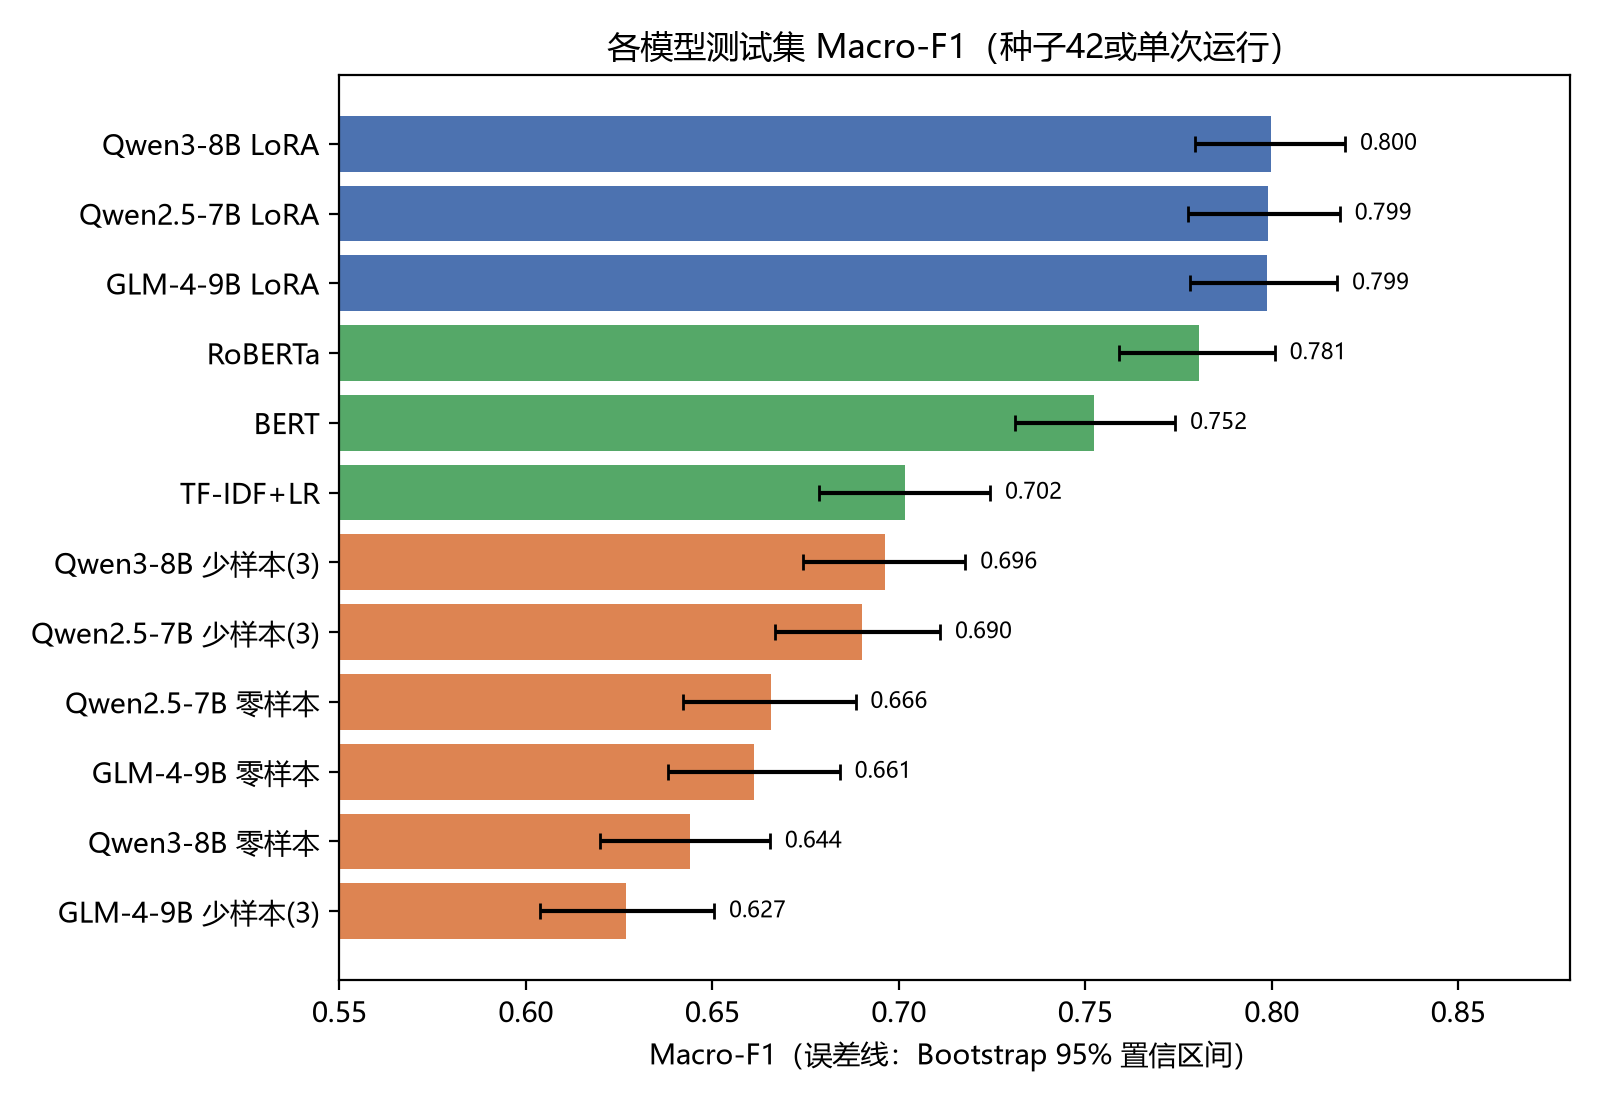
\includegraphics[width=\linewidth,height=0.80\textheight,keepaspectratio]{figures/fig_model_comparison.png}
\caption{各模型种子 42 或单次运行的 Macro-\allowbreak{}F1（柱高与 Bootstrap 95\% 区间对应同一次运行）}\label{fig:4-1}\end{figure}

综合表~\ref{tab:4-1} 与表~\ref{tab:4-2} 可以得出以下几点：

第一，LoRA 微调后的三个大模型取得了最好的效果，Macro-F1 在 0.798～0.807 之间，准确率在 81.8\%～82.6\% 之间。其中 Qwen2.5-7B 的平均 Macro-F1 最高（0.807），但三个大模型之间的差距不超过 0.01。

第二，不经微调的大模型表现较差。三个模型零样本的 Macro-F1 只有 0.644～0.666，甚至低于最简单的 TF-IDF + 逻辑回归（0.702）。这与 DISC-FinLLM\cite{ref33} 等研究报告的通用大模型在 FinFE 上准确率约为 60\%～69\% 的结论一致，与通用提示难以直接匹配本任务标签分布的解释相容，但并不能单凭分数定位为模型缺少某类知识。

第三，提供示例的作用有限且不稳定。每类给出 3 个示例时，Qwen3-8B 的 Macro-F1 从 0.644 提高到 0.696，Qwen2.5-7B 从 0.666 提高到 0.690，而 GLM-4-9B 反而从 0.661 下降到 0.627。每类只给 1 个示例时，GLM-4-9B 同样下降（0.630），Qwen2.5-7B 基本不变（0.666）。在当前固定提示和示例抽样下，少样本收益因模型而异；没有重复抽取示例，不能将这一结果外推为提示方法普遍不可靠。

第四，所有模型在中性类上的 F1 都明显低于另外两类。即使是表现最好的模型，中性类 F1 也只有 0.707，比积极类低约 17 个百分点。结合 3.3 节的描述性统计，中性评论多为提问或客观陈述，与带有轻微情绪的消极、积极评论边界模糊；数据清洗中发现的 228 条跨文件标签不一致样本也说明，人工标注在这些样本上同样存在分歧。

\FloatBarrier\subsection{显著性检验}

\subsubsection{McNemar 检验}

表~\ref{tab:4-3} 列出了 TF-IDF + 逻辑回归、RoBERTa 和三个 LoRA 大模型（均取种子 42 的运行）两两之间的 McNemar 检验结果，p 值经 Holm 方法校正。

\begin{table}[htbp]
\centering
\begin{minipage}{\textwidth}
\setlength{\tabcolsep}{3pt}
\renewcommand{\arraystretch}{1.16}
\setstretch{1.0}\fontsize{10.5}{13.5}\selectfont
\caption{McNemar 检验结果（Holm 校正）}\label{tab:4-3}
\begin{tabular}{>{\raggedright\arraybackslash}p{\dimexpr 0.200000\linewidth-2.800000\tabcolsep\relax}>{\raggedright\arraybackslash}p{\dimexpr 0.200000\linewidth-2.800000\tabcolsep\relax}>{\raggedright\arraybackslash}p{\dimexpr 0.120000\linewidth-1.680000\tabcolsep\relax}>{\raggedright\arraybackslash}p{\dimexpr 0.120000\linewidth-1.680000\tabcolsep\relax}>{\raggedright\arraybackslash}p{\dimexpr 0.120000\linewidth-1.680000\tabcolsep\relax}>{\raggedright\arraybackslash}p{\dimexpr 0.120000\linewidth-1.680000\tabcolsep\relax}>{\raggedright\arraybackslash}p{\dimexpr 0.120000\linewidth-1.680000\tabcolsep\relax}}
\toprule
\textbf{模型 A} & \textbf{模型 B} & \textbf{A 对 B 错} & \textbf{A 错 B 对} & \textbf{$\chi^{2}$} & \textbf{原始 p 值} & \textbf{校正后 p 值} \\
\midrule
TF-\allowbreak{}IDF+LR & RoBERTa & 101 & 223 & 45.19 & 1.8$\times$10$^{-11}$ & 1.3$\times$10$^{-10}$ \\
TF-\allowbreak{}IDF+LR & Qwen3-\allowbreak{}8B LoRA & 109 & 257 & 59.04 & 1.5$\times$10$^{-14}$ & 1.5$\times$10$^{-13}$ \\
TF-\allowbreak{}IDF+LR & Qwen2.5-\allowbreak{}7B LoRA & 112 & 255 & 54.94 & 1.2$\times$10$^{-13}$ & 1.1$\times$10$^{-12}$ \\
TF-\allowbreak{}IDF+LR & GLM-\allowbreak{}4-\allowbreak{}9B LoRA & 118 & 263 & 54.43 & 1.6$\times$10$^{-13}$ & 1.3$\times$10$^{-12}$ \\
RoBERTa & Qwen3-\allowbreak{}8B LoRA & 97 & 123 & 2.84 & 0.092 & 0.551 \\
RoBERTa & Qwen2.5-\allowbreak{}7B LoRA & 83 & 104 & 2.14 & 0.144 & 0.695 \\
RoBERTa & GLM-\allowbreak{}4-\allowbreak{}9B LoRA & 99 & 122 & 2.19 & 0.139 & 0.695 \\
Qwen3-\allowbreak{}8B LoRA & Qwen2.5-\allowbreak{}7B LoRA & 82 & 77 & 0.10 & 0.751 & 1.000 \\
Qwen3-\allowbreak{}8B LoRA & GLM-\allowbreak{}4-\allowbreak{}9B LoRA & 85 & 82 & 0.02 & 0.877 & 1.000 \\
Qwen2.5-\allowbreak{}7B LoRA & GLM-\allowbreak{}4-\allowbreak{}9B LoRA & 87 & 89 & 0.01 & 0.940 & 1.000 \\
\bottomrule\end{tabular}
\end{minipage}
\end{table}

结果显示：RoBERTa 和三个大模型均极显著优于 TF-IDF 基线；三个大模型之间差异很小，两个模型判断不一致的样本中，双方各对一半左右，校正后 p 值均为 1；大模型与 RoBERTa 相比，虽然``大模型对、RoBERTa 错''的样本多于反向情况（如 123 对 97），但即使不做校正也未达到 0.05 的显著性水平，校正后 p 值在 0.55～0.70 之间。

\subsubsection{配对 Bootstrap}

McNemar 检验只关注准确率。表~\ref{tab:4-4} 给出以 Macro-F1 为指标的配对 Bootstrap 结果（B = 50000，种子 42 的模型预测）。表中展示六对主要比较，但多重比较家族包含五模型的全部十对，并未因展示范围而缩小。

\begin{table}[htbp]
\centering
\begin{minipage}{\textwidth}
\setlength{\tabcolsep}{3pt}
\renewcommand{\arraystretch}{1.16}
\setstretch{1.0}\fontsize{10.5}{13.5}\selectfont
\caption{配对 Bootstrap：Macro-\allowbreak{}F1 差值与区间}\label{tab:4-4}
\begin{tabular}{>{\raggedright\arraybackslash}p{\dimexpr 0.200000\linewidth-2.000000\tabcolsep\relax}>{\raggedright\arraybackslash}p{\dimexpr 0.200000\linewidth-2.000000\tabcolsep\relax}>{\raggedright\arraybackslash}p{\dimexpr 0.120000\linewidth-1.200000\tabcolsep\relax}>{\raggedright\arraybackslash}p{\dimexpr 0.240000\linewidth-2.400000\tabcolsep\relax}>{\raggedright\arraybackslash}p{\dimexpr 0.240000\linewidth-2.400000\tabcolsep\relax}}
\toprule
\textbf{模型 A} & \textbf{模型 B} & \textbf{差值（A $-$ B）} & \textbf{单比较 95\% 区间} & \textbf{Bonferroni 调整区间} \\
\midrule
RoBERTa & Qwen3-\allowbreak{}8B LoRA & -\allowbreak{}0.01929 & [-\allowbreak{}0.03885, 0.00012] & [-\allowbreak{}0.04725, 0.00892] \\
RoBERTa & Qwen2.5-\allowbreak{}7B LoRA & -\allowbreak{}0.01829 & [-\allowbreak{}0.03608, -\allowbreak{}0.00079] & [-\allowbreak{}0.04357, 0.00690] \\
RoBERTa & GLM-\allowbreak{}4-\allowbreak{}9B LoRA & -\allowbreak{}0.01816 & [-\allowbreak{}0.03785, 0.00126] & [-\allowbreak{}0.04667, 0.01032] \\
Qwen3-\allowbreak{}8B LoRA & Qwen2.5-\allowbreak{}7B LoRA & 0.00099 & [-\allowbreak{}0.01554, 0.01713] & [-\allowbreak{}0.02244, 0.02414] \\
Qwen3-\allowbreak{}8B LoRA & GLM-\allowbreak{}4-\allowbreak{}9B LoRA & 0.00112 & [-\allowbreak{}0.01570, 0.01808] & [-\allowbreak{}0.02305, 0.02547] \\
Qwen2.5-\allowbreak{}7B LoRA & GLM-\allowbreak{}4-\allowbreak{}9B LoRA & 0.00013 & [-\allowbreak{}0.01706, 0.01746] & [-\allowbreak{}0.02440, 0.02465] \\
\bottomrule\end{tabular}
\end{minipage}
\end{table}

两个 Qwen 模型和 GLM 相对 RoBERTa 的 F1 点估计均高约 1.8～1.9 个百分点。在未调整区间中，仅 Qwen2.5 的区间不包含 0；经十对比较的 Bonferroni 调整后，三个 LoRA 对 RoBERTa 的区间均包含 0。Qwen3 的未调整区间边界非常接近 0，提示结论对重抽样误差敏感，不宜用单个区间是否刚好跨 0 强调``边缘显著''。三个 LoRA 模型之间的调整区间也均包含 0，未检出差异不等于证明效果相同。

\subsubsection{多种子方差分析}

表~\ref{tab:4-5} 为五个多种子模型的 Macro-F1 方差分析结果。

\begin{table}[htbp]
\centering
\begin{minipage}{\textwidth}
\setlength{\tabcolsep}{3pt}
\renewcommand{\arraystretch}{1.16}
\setstretch{1.0}\fontsize{10.5}{13.5}\selectfont
\caption{多种子 Macro-\allowbreak{}F1 方差分析}\label{tab:4-5}
\begin{tabular}{>{\raggedright\arraybackslash}p{\dimexpr 0.333333\linewidth-2.000000\tabcolsep\relax}>{\raggedright\arraybackslash}p{\dimexpr 0.333333\linewidth-2.000000\tabcolsep\relax}>{\raggedright\arraybackslash}p{\dimexpr 0.333333\linewidth-2.000000\tabcolsep\relax}}
\toprule
\textbf{检验} & \textbf{统计量} & \textbf{p 值} \\
\midrule
Levene 方差齐性检验 & W = 0.262 & 0.896 \\
单因素方差分析（5 组） & F = 31.87 & 1.1$\times$10$^{-5}$ \\
Welch 方差分析（5 组） & F = 19.84 & 0.004 \\
单因素方差分析（仅三个 LoRA 大模型） & F = 2.78 & 0.140 \\
\bottomrule\end{tabular}
\end{minipage}
\end{table}

Levene 检验未检出方差差异（p = 0.896），但每组仅 3 次，不能据此证明方差相等，单因素方差分析和 Welch 方差分析均显示五个模型的平均 Macro-F1 存在显著差异。Tukey HSD 事后比较（表~\ref{tab:4-6}）表明：三个 LoRA 大模型均显著优于 RoBERTa（平均高 2.0～2.9 个百分点，p \textless{} 0.03），RoBERTa 显著优于 BERT（p = 0.017），而三个大模型之间两两差异均不显著（p \textgreater{} 0.38）。

\begin{table}[htbp]
\centering
\begin{minipage}{\textwidth}
\setlength{\tabcolsep}{3pt}
\renewcommand{\arraystretch}{1.16}
\setstretch{1.0}\fontsize{10.5}{13.5}\selectfont
\caption{Tukey HSD 事后比较（均值差 = 组 2 $-$ 组 1）}\label{tab:4-6}
\begin{tabular}{>{\raggedright\arraybackslash}p{\dimexpr 0.200000\linewidth-2.000000\tabcolsep\relax}>{\raggedright\arraybackslash}p{\dimexpr 0.200000\linewidth-2.000000\tabcolsep\relax}>{\raggedright\arraybackslash}p{\dimexpr 0.120000\linewidth-1.200000\tabcolsep\relax}>{\raggedright\arraybackslash}p{\dimexpr 0.140000\linewidth-1.400000\tabcolsep\relax}>{\raggedright\arraybackslash}p{\dimexpr 0.340000\linewidth-3.400000\tabcolsep\relax}}
\toprule
\textbf{组 1} & \textbf{组 2} & \textbf{均值差} & \textbf{调整后 p 值} & \textbf{95\% 置信区间} \\
\midrule
BERT & RoBERTa & 0.020 & 0.017 & [0.004, 0.037] \\
RoBERTa & Qwen3-\allowbreak{}8B LoRA & 0.023 & 0.008 & [0.006, 0.040] \\
RoBERTa & Qwen2.5-\allowbreak{}7B LoRA & 0.029 & 0.001 & [0.012, 0.046] \\
RoBERTa & GLM-\allowbreak{}4-\allowbreak{}9B LoRA & 0.020 & 0.021 & [0.003, 0.036] \\
Qwen3-\allowbreak{}8B LoRA & Qwen2.5-\allowbreak{}7B LoRA & 0.006 & 0.754 & [$-$0.011, 0.023] \\
GLM-\allowbreak{}4-\allowbreak{}9B LoRA & Qwen3-\allowbreak{}8B LoRA & 0.003 & 0.958 & [$-$0.013, 0.020] \\
GLM-\allowbreak{}4-\allowbreak{}9B LoRA & Qwen2.5-\allowbreak{}7B LoRA & 0.010 & 0.389 & [$-$0.007, 0.026] \\
\bottomrule\end{tabular}
\end{minipage}
\end{table}

\subsubsection{检验结果的综合解读}

不同方法考察的随机性与评价指标并不相同。多种子 ANOVA 和 Tukey 比较条件于当前训练、验证和测试划分，反映有限训练重复间的差异；McNemar 与配对 Bootstrap 条件于种子 42 的训练结果，考察测试样本的配对抽样误差，且分别针对准确率和 Macro-F1。前者的显著结果不能替代后者，也不能替代面向新数据的验证。

在所考察的三个种子中，三个 LoRA 模型的 F1 点估计均高于 RoBERTa，平均差为约 2.0～2.9 个百分点；但种子 42 的 McNemar 检验和配对 Bootstrap 在各自的多重比较调整后均未检出显著优势。因此，本文将结论限定为``在本数据划分和三个训练种子中观察到一致较高的点估计''，不推广为对新样本的稳定优越性。三个 LoRA 模型之间未检出差异，也不构成等效性结论。

\FloatBarrier\subsection{校准分析}

原始概率指标与温度交叉拟合结果分别见表~\ref{tab:4-7}、表~\ref{tab:4-8}，可靠性图见图~\ref{fig:4-2}。

\begin{table}[htbp]
\centering
\begin{minipage}{\textwidth}
\setlength{\tabcolsep}{3pt}
\renewcommand{\arraystretch}{1.16}
\setstretch{1.0}\fontsize{10.5}{13.5}\selectfont
\caption{原始概率的校准指标（种子 42 或单次）}\label{tab:4-7}
\begin{tabular}{>{\raggedright\arraybackslash}p{\dimexpr 0.300000\linewidth-3.600000\tabcolsep\relax}>{\raggedright\arraybackslash}p{\dimexpr 0.140000\linewidth-1.680000\tabcolsep\relax}>{\raggedright\arraybackslash}p{\dimexpr 0.140000\linewidth-1.680000\tabcolsep\relax}>{\raggedright\arraybackslash}p{\dimexpr 0.140000\linewidth-1.680000\tabcolsep\relax}>{\raggedright\arraybackslash}p{\dimexpr 0.140000\linewidth-1.680000\tabcolsep\relax}>{\raggedright\arraybackslash}p{\dimexpr 0.140000\linewidth-1.680000\tabcolsep\relax}}
\toprule
\textbf{模型} & \textbf{平均置信度} & \textbf{准确率} & \textbf{ECE} & \textbf{Brier} & \textbf{NLL} \\
\midrule
TF-\allowbreak{}IDF+LR & 0.777 & 0.734 & 0.045 & 0.367 & 0.651 \\
RoBERTa & 0.830 & 0.806 & 0.031 & 0.276 & 0.493 \\
Qwen3-\allowbreak{}8B 零样本 & 0.964 & 0.671 & 0.294 & 0.610 & 3.330 \\
Qwen3-\allowbreak{}8B LoRA & 0.880 & 0.821 & 0.061 & 0.266 & 0.486 \\
Qwen2.5-\allowbreak{}7B LoRA & 0.852 & 0.818 & 0.035 & 0.261 & 0.474 \\
GLM-\allowbreak{}4-\allowbreak{}9B LoRA & 0.900 & 0.819 & 0.085 & 0.281 & 0.527 \\
\bottomrule\end{tabular}
\par\vspace{3pt}{\fontsize{10}{12.5}\selectfont 注：由历史六位小数概率计算，NLL 截断下限为 1e-\allowbreak{}12；零样本敏感性见本节。\par}
\end{minipage}
\end{table}

\begin{table}[htbp]
\centering
\begin{minipage}{\textwidth}
\setlength{\tabcolsep}{3pt}
\renewcommand{\arraystretch}{1.16}
\setstretch{1.0}\fontsize{10.5}{13.5}\selectfont
\caption{温度交叉拟合后的校准指标}\label{tab:4-8}
\begin{tabular}{>{\raggedright\arraybackslash}p{\dimexpr 0.400000\linewidth-3.200000\tabcolsep\relax}>{\raggedright\arraybackslash}p{\dimexpr 0.200000\linewidth-1.600000\tabcolsep\relax}>{\raggedright\arraybackslash}p{\dimexpr 0.200000\linewidth-1.600000\tabcolsep\relax}>{\raggedright\arraybackslash}p{\dimexpr 0.200000\linewidth-1.600000\tabcolsep\relax}}
\toprule
\textbf{模型} & \textbf{温度 T} & \textbf{缩放后 ECE} & \textbf{缩放后 NLL} \\
\midrule
TF-\allowbreak{}IDF+LR & 1.24 & 0.023 & 0.640 \\
RoBERTa & 1.09 & 0.018 & 0.492 \\
Qwen3-\allowbreak{}8B 零样本 & 9.85 & 0.030 & 0.811 \\
Qwen3-\allowbreak{}8B LoRA & 1.41 & 0.013 & 0.458 \\
Qwen2.5-\allowbreak{}7B LoRA & 1.19 & 0.019 & 0.468 \\
GLM-\allowbreak{}4-\allowbreak{}9B LoRA & 1.60 & 0.030 & 0.469 \\
\bottomrule\end{tabular}
\par\vspace{3pt}{\fontsize{10}{12.5}\selectfont 注：T 为五折拟合值均值，不是经独立验证的部署温度；缩放前后准确率不变，NLL 使用同一截断约定。\par}
\end{minipage}
\end{table}

\begin{figure}[htbp]\centering
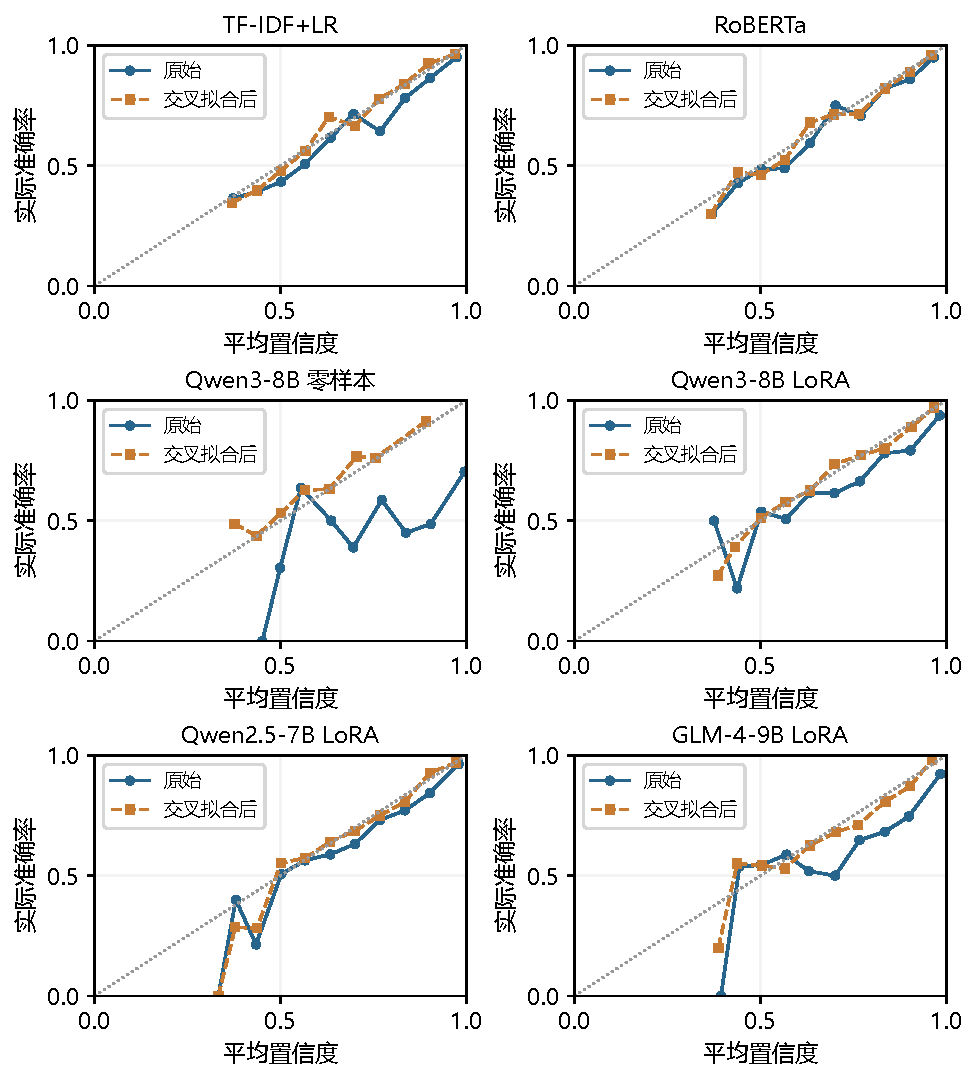
\includegraphics[width=\linewidth,height=0.80\textheight,keepaspectratio]{figures/fig_reliability.pdf}
\caption{可靠性图（对角线表示完美校准，曲线位于对角线下方表示过度自信）}\label{fig:4-2}\end{figure}

结果显示出三个特点：

第一，未经微调的大模型严重过度自信。Qwen3-8B 零样本的平均置信度高达 96.4\%，实际准确率只有 67.1\%，ECE 为 0.294，NLL 为 3.33，在当前截断约定下得到平均温度 T = 9.85；置信度与准确率之间的差距支持过度自信判断，但 NLL 和温度的具体数值需结合存储精度限制解释。

第二，LoRA 微调大幅改善了校准，但大模型仍比 RoBERTa 更加过度自信。三个 LoRA 大模型的 ECE 在 0.035～0.085 之间，平均置信度均高于准确率，最优温度均大于 1；其中 GLM-4-9B 最明显（置信度 90.0\%，准确率 81.9\%）。RoBERTa 的 ECE 为 0.031，是未校准时最低的。这说明训练后的概率仍需要单独评估，与第 2 章区分判别能力和不确定性评估的思路相一致。值得注意的是，在 Brier 分数和 NLL 这两个同时反映判别能力和校准的指标上，Qwen 系列的 LoRA 模型仍优于 RoBERTa。

第三，在当前测试分布内，五折温度交叉拟合降低了 ECE。各模型的 ECE 降到 0.013～0.030，其中 Qwen3-8B LoRA 从 0.061 降到 0.013，是本表 ECE 最低者。对单个样本，正温度不改变其类别 logits 的大小顺序，因此不改变预测类别、准确率和 Macro-F1；这并不意味着跨样本的置信度排序一定不变。本文的选择性预测仍使用原始概率排序，没有把校准后的结果与其混用。

需要特别说明，Qwen3 零样本的 1713 条预测中有 91 条真实类别概率在历史 CSV 中为零。仅将截断下限从 1e-12 改为 1e-8 或 1e-6，NLL 就由 3.3301 变为 2.8408 或 2.5962，平均温度由 9.8543 变为 7.5518 或 6.5507。上述变化是数值敏感性，不是不同模型效果；任何一个截断下限都不能恢复原始 logits。本轮未重新推理，因此保留原表并明确其约定，后续应保存高精度概率或 logits 后再核验零样本 NLL、温度及极端分数并列。Qwen3 LoRA 本次没有零概率，在这些下限下指标不变；不能把零样本敏感性泛化到全部模型。完整结果见 outputs/analysis/probability\_precision.csv。

\FloatBarrier\subsection{选择性预测}

表~\ref{tab:4-9} 和图~\ref{fig:4-3} 给出了各模型的选择性预测结果。

\begin{table}[htbp]
\centering
\begin{minipage}{\textwidth}
\setlength{\tabcolsep}{3pt}
\renewcommand{\arraystretch}{1.16}
\setstretch{1.0}\fontsize{10.5}{13.5}\selectfont
\caption{选择性预测结果（种子 42）}\label{tab:4-9}
\begin{tabular}{>{\raggedright\arraybackslash}p{\dimexpr 0.280000\linewidth-3.920000\tabcolsep\relax}>{\raggedright\arraybackslash}p{\dimexpr 0.100000\linewidth-1.400000\tabcolsep\relax}>{\raggedright\arraybackslash}p{\dimexpr 0.100000\linewidth-1.400000\tabcolsep\relax}>{\raggedright\arraybackslash}p{\dimexpr 0.130000\linewidth-1.820000\tabcolsep\relax}>{\raggedright\arraybackslash}p{\dimexpr 0.130000\linewidth-1.820000\tabcolsep\relax}>{\raggedright\arraybackslash}p{\dimexpr 0.130000\linewidth-1.820000\tabcolsep\relax}>{\raggedright\arraybackslash}p{\dimexpr 0.130000\linewidth-1.820000\tabcolsep\relax}}
\toprule
\textbf{模型} & \textbf{AURC} & \textbf{E-\allowbreak{}AURC} & \textbf{覆盖 50\% 准确率} & \textbf{覆盖 80\% 准确率} & \textbf{覆盖 90\% 准确率} & \textbf{全部作答准确率} \\
\midrule
TF-\allowbreak{}IDF+LR & 0.114 & 0.075 & 0.895 & 0.806 & 0.772 & 0.734 \\
RoBERTa & 0.074 & 0.054 & 0.943 & 0.880 & 0.846 & 0.806 \\
Qwen3-\allowbreak{}8B 零样本 & 0.200 & 0.138 & 0.804 & 0.722 & 0.693 & 0.671 \\
Qwen3-\allowbreak{}8B LoRA & 0.060 & 0.043 & 0.957 & 0.891 & 0.859 & 0.821 \\
Qwen2.5-\allowbreak{}7B LoRA & 0.060 & 0.042 & 0.961 & 0.888 & 0.856 & 0.818 \\
GLM-\allowbreak{}4-\allowbreak{}9B LoRA & 0.062 & 0.045 & 0.954 & 0.882 & 0.849 & 0.819 \\
\bottomrule\end{tabular}
\end{minipage}
\end{table}

\begin{figure}[htbp]\centering
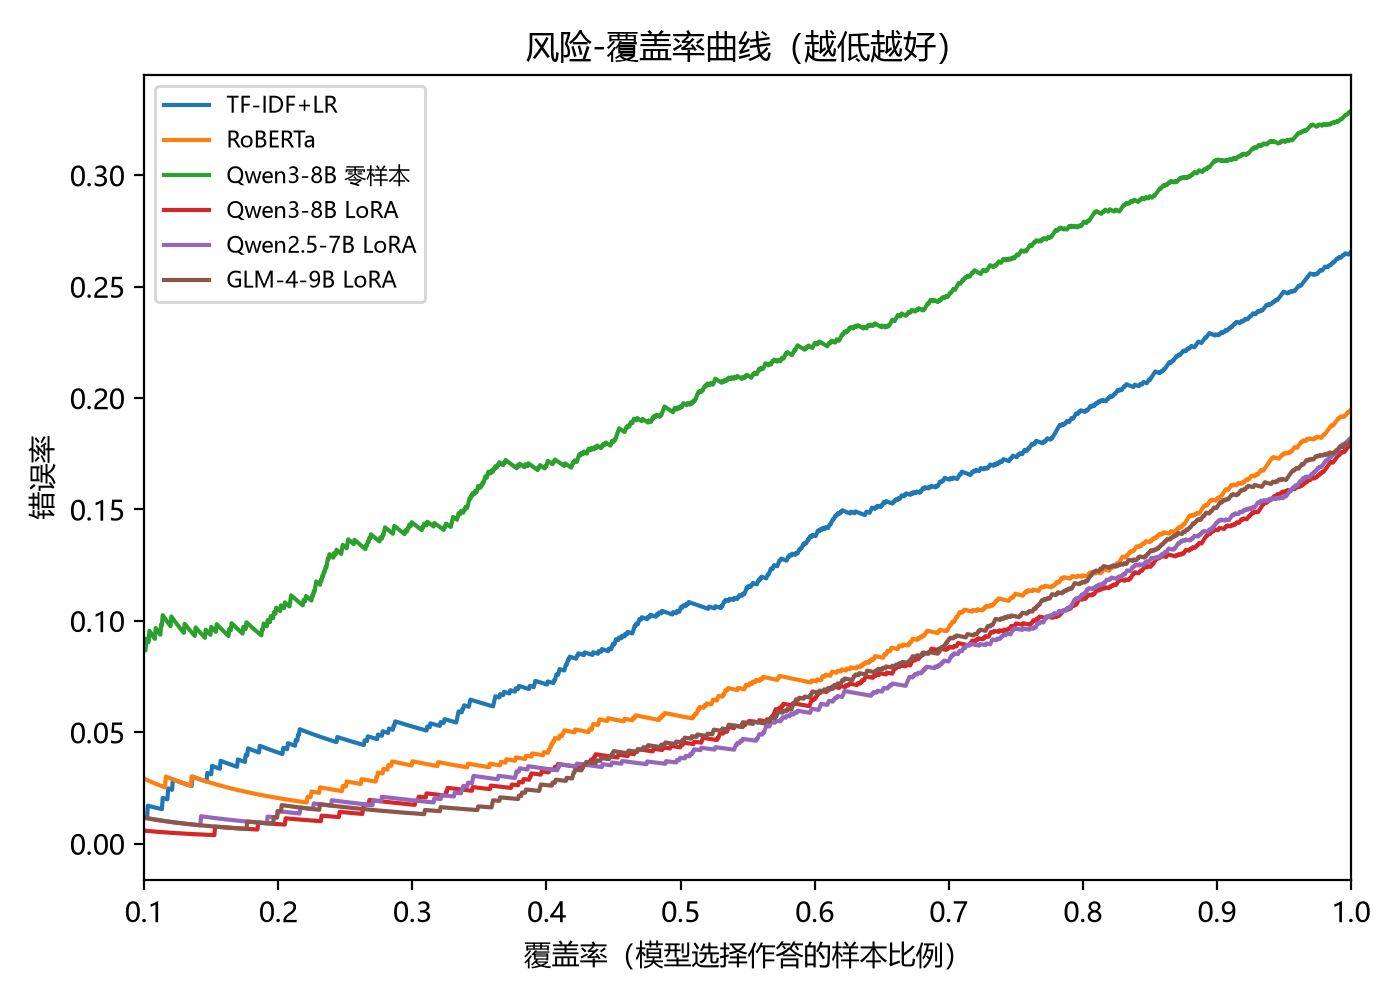
\includegraphics[width=\linewidth,height=0.80\textheight,keepaspectratio]{figures/fig_risk_coverage.png}
\caption{风险-\allowbreak{}覆盖率曲线}\label{fig:4-3}\end{figure}

三个 LoRA 大模型的 AURC 约为 0.060，明显低于 RoBERTa（0.074）和 TF-IDF（0.114）。E-AURC 的排序与之相同，说明大模型的优势不仅来自更高的整体准确率，也来自置信度对对错更好的区分能力。换言之，大模型虽然整体上过度自信，但它``更有把握''的样本确实更可能判断正确。

从应用角度看，若只让 Qwen2.5-7B LoRA 回答置信度最高的 50\% 评论，准确率可达 96.1\%；覆盖 80\% 时准确率仍有 88.8\%。这为部分自动化提供了数据内参考；实际阈值仍须在独立校准集确定，再在新样本上验证，本文未验证部署错误率或实际人工成本。

\FloatBarrier\subsection{消融实验}

为分析训练样本量、LoRA 秩和量化精度对效果的影响，本文以 Qwen3-8B 为对象、固定种子 42 进行了消融实验，结果见表~\ref{tab:4-10} 和图~\ref{fig:4-4}。训练样本量实验中，由于样本较少，训练轮数由 2 轮增加到 3 轮。

\begin{table}[htbp]
\centering
\begin{minipage}{\textwidth}
\setlength{\tabcolsep}{3pt}
\renewcommand{\arraystretch}{1.16}
\setstretch{1.0}\fontsize{10.5}{13.5}\selectfont
\caption{消融实验结果（Qwen3-\allowbreak{}8B，种子 42）}\label{tab:4-10}
\begin{tabular}{>{\raggedright\arraybackslash}p{\dimexpr 0.200000\linewidth-2.000000\tabcolsep\relax}>{\raggedright\arraybackslash}p{\dimexpr 0.200000\linewidth-2.000000\tabcolsep\relax}>{\raggedright\arraybackslash}p{\dimexpr 0.200000\linewidth-2.000000\tabcolsep\relax}>{\raggedright\arraybackslash}p{\dimexpr 0.200000\linewidth-2.000000\tabcolsep\relax}>{\raggedright\arraybackslash}p{\dimexpr 0.200000\linewidth-2.000000\tabcolsep\relax}}
\toprule
\textbf{消融因素} & \textbf{设置} & \textbf{Macro-\allowbreak{}F1} & \textbf{准确率} & \textbf{峰值显存} \\
\midrule
训练样本量 & 0（零样本） & 0.644 & 0.671 & — \\
训练样本量 & 500 & 0.766 & 0.790 & — \\
训练样本量 & 1000 & 0.772 & 0.788 & — \\
训练样本量 & 2000 & 0.770 & 0.790 & — \\
训练样本量 & 4000 & 0.789 & 0.809 & — \\
训练样本量 & 8802（全部） & 0.800 & 0.821 & 18.3 GB \\
LoRA 秩 & r = 4（1091 万参数） & 0.804 & 0.825 & 17.9 GB \\
LoRA 秩 & r = 8（2182 万参数） & 0.809 & 0.828 & 18.1 GB \\
LoRA 秩 & r = 16（4365 万参数） & 0.800 & 0.821 & 18.3 GB \\
LoRA 秩 & r = 32（8729 万参数） & 0.798 & 0.818 & 18.9 GB \\
量化精度 & 16 位（bf16） & 0.800 & 0.821 & 18.3 GB \\
量化精度 & 4 位（QLoRA） & 0.807 & 0.828 & 11.2 GB \\
\bottomrule\end{tabular}
\end{minipage}
\end{table}

\begin{figure}[htbp]\centering
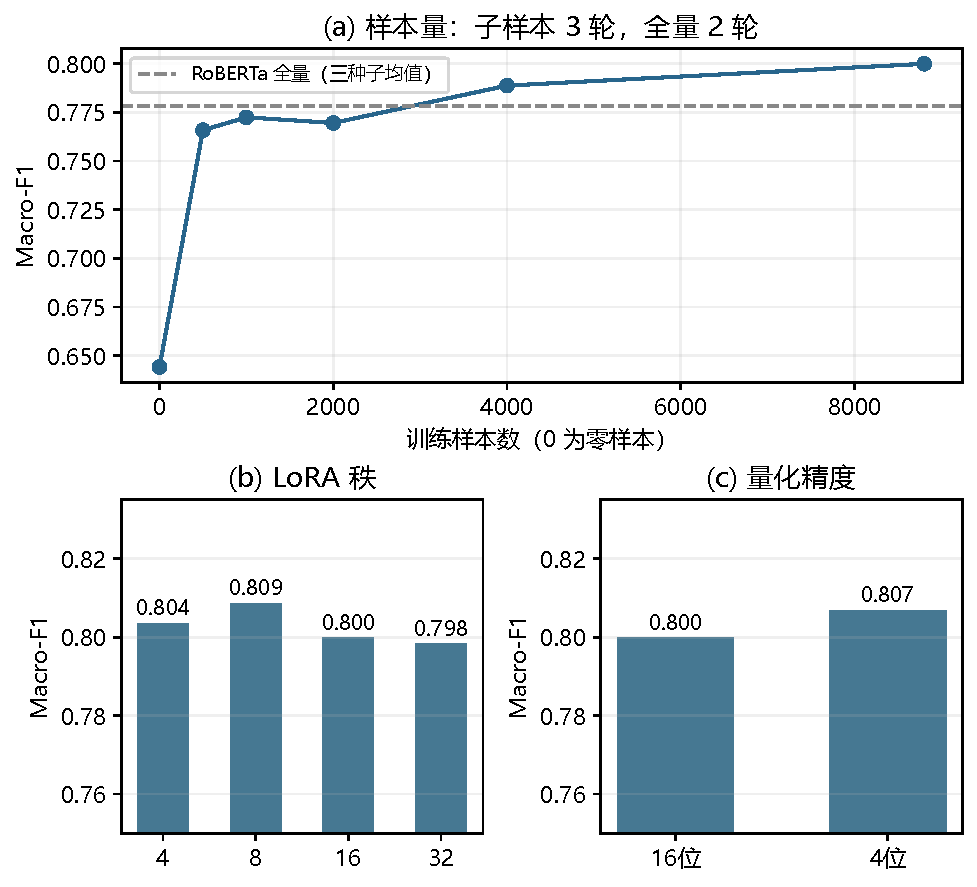
\includegraphics[width=\linewidth,height=0.80\textheight,keepaspectratio]{figures/fig_ablation.pdf}
\caption{Qwen3-\allowbreak{}8B LoRA 消融实验}\label{fig:4-4}\end{figure}

\textbf{训练样本量。} 只用 500 条样本微调，Macro-F1 就从零样本的 0.644 提高到 0.766，接近用全部 8802 条数据训练的 RoBERTa（0.778）。此后继续增加数据，效果提升逐渐放缓：从 500 条增加到 8802 条，数据量增加约 17 倍，Macro-F1 只提高 3.4 个百分点。这说明大模型只需少量标注数据就能适应任务，在标注成本较高的金融场景中有实际意义。

\textbf{LoRA 秩。} 秩从 4 增加到 32，可训练参数增加 8 倍，Macro-F1 却在 0.798～0.809 之间小幅波动，没有随参数增加而提高。考虑到同一模型不同种子之间的标准差约为 0.002～0.007，且每个秩只运行了一次，当前只能描述各秩的单次结果接近；缺少各秩多次重复和等效性检验，不能据此证明各秩等效或任务只需要某个固定更新量。

\textbf{量化精度。} 4-bit 量化将训练峰值显存从 18.3 GB 降到 11.2 GB，降幅约 39\%，而 Macro-F1 没有下降（0.807 对 0.800），代价是训练时间从 38 分钟增加到 44 分钟。这里的显存指标来自框架的峰值已分配内存，不等于整卡实际占用；因此该结果提示较低资源配置的可行性，但不能保证任意 12 GB 显卡及软件环境均可运行，也不能由一次实验证明两种精度等效。

\FloatBarrier\subsection{评估曝光与清洗策略比较}

本文保留了未清洗策略的实验：原始训练文件随机划出 10\% 作为验证集，在其余样本上训练 TF-IDF+LR 和 RoBERTa（3 个种子），再评估原始 eval\_list 的 2020 条记录。原始训练文件中的记录不都参与参数优化，因此区分两种曝光口径：

（1）以原始训练文件（包含后来划出的验证集）为基准，seen\_same / seen\_diff / unseen 为 868 / 229 / 923； （2）只以实际优化训练集为基准，三组为 787 / 202 / 1031。其中 108 条评估记录仅在验证集出现，不在优化训练集出现。验证集参与模型选择，仍属于开发数据曝光，但不能直接称为训练时``背答案''。

表~\ref{tab:4-11} 采用第二种口径，RoBERTa 报告三个种子的平均指标。这里的``训练中未见''包括验证曝光记录，不等于完全独立于模型开发。

\begin{table}[htbp]
\centering
\begin{minipage}{\textwidth}
\setlength{\tabcolsep}{3pt}
\renewcommand{\arraystretch}{1.16}
\setstretch{1.0}\fontsize{10.5}{13.5}\selectfont
\caption{按实际优化训练集曝光分组的评估结果}\label{tab:4-11}
\begin{tabular}{>{\raggedright\arraybackslash}p{\dimexpr 0.300000\linewidth-3.600000\tabcolsep\relax}>{\raggedright\arraybackslash}p{\dimexpr 0.100000\linewidth-1.200000\tabcolsep\relax}>{\raggedright\arraybackslash}p{\dimexpr 0.150000\linewidth-1.800000\tabcolsep\relax}>{\raggedright\arraybackslash}p{\dimexpr 0.150000\linewidth-1.800000\tabcolsep\relax}>{\raggedright\arraybackslash}p{\dimexpr 0.150000\linewidth-1.800000\tabcolsep\relax}>{\raggedright\arraybackslash}p{\dimexpr 0.150000\linewidth-1.800000\tabcolsep\relax}}
\toprule
\textbf{测试子集} & \textbf{样本数} & \textbf{TF-\allowbreak{}IDF+LR 准确率} & \textbf{TF-\allowbreak{}IDF+LR Macro-\allowbreak{}F1} & \textbf{RoBERTa 准确率} & \textbf{RoBERTa Macro-\allowbreak{}F1} \\
\midrule
原始全部评估集 & 2020 & 0.7703 & 0.7547 & 0.7881 & 0.7734 \\
优化训练中见过且含同标签 & 787 & 0.9975 & 0.9974 & 0.9399 & 0.9371 \\
优化训练中见过但仅含不同标签 & 202 & 0.0000 & 0.0000 & 0.1881 & 0.1915 \\
优化训练中未见（含验证曝光） & 1031 & 0.7478 & 0.6767 & 0.7898 & 0.7411 \\
\bottomrule\end{tabular}
\end{minipage}
\end{table}

对实际优化训练中存在相同标签的原句，TF-IDF 的准确率为 99.75\%，RoBERTa 为 93.99\%；在优化训练中仅有不同标签的子集上，两者分别为 0\% 和 18.81\%。这与模型对已曝光文本的记忆相一致，但分组并非随机，样本难度和类别构成也不同，不能用组间差值识别纯泄漏效应。

为与原分析口径对照，原始训练文件意义下的全体评估与 unseen 子集上，TF-IDF 的 Macro-F1 分别为 0.7547 与 0.6733，差约 8.14 个百分点；RoBERTa 分别为 0.7734 与 0.7400，差约 3.34 个百分点。这些是不同样本总体的描述差：unseen 子集积极类占 63.1\%，seen\_same 中仅占 28.1\%，Macro-F1 也不满足按子集比例线性加权。因此不将 8.14 个百分点称为纯泄漏造成的虚高，也不把不同子集中的模型差距变化称为``真实差距被缩小''。

进一步将两种训练策略严格对齐到同样的 845 条共同未曝光文本及相同标签上，TF-IDF 的 Macro-F1 为 0.6543（未清洗训练）和 0.6583（清洗后训练）；RoBERTa 三种子均值为 0.7309 和 0.7392。这一比较没有观察到 F1 点估计下降，但尚未作等效性检验，且同时改变了去重、冲突处理和训练样本构成，只能解释为清洗策略的整体比较。若要估计单独的泄漏因果效应，需要固定测试样本并控制其他处理因素。详细分组和共同样本结果分别见 outputs/analysis/leakage.csv 与 outputs/analysis/leakage\_matched.csv。

\FloatBarrier\subsection{重复记录一致性与噪声情景分析}

原始 FinFE 两个文件中有 5575 个规范化文本出现两次及以上，对每个文本的全部记录作两两配对，共得到 6048 对。文件不提供标注者 ID、独立复标过程或金标准，因此下文描述的是重复记录的一致性，而非已经确认的独立人工复标可靠性。

\begin{table}[htbp]
\centering
\begin{minipage}{\textwidth}
\setlength{\tabcolsep}{3pt}
\renewcommand{\arraystretch}{1.16}
\setstretch{1.0}\fontsize{10.5}{13.5}\selectfont
\caption{重复记录的标签一致性分析}\label{tab:4-12}
\begin{tabular}{>{\raggedright\arraybackslash}p{\dimexpr 0.460000\linewidth-1.840000\tabcolsep\relax}>{\raggedright\arraybackslash}p{\dimexpr 0.540000\linewidth-2.160000\tabcolsep\relax}}
\toprule
\textbf{指标} & \textbf{数值} \\
\midrule
重复文本数 /\allowbreak{} 记录配对数 & 5575 /\allowbreak{} 6048 \\
配对一致率 p\_\allowbreak{}o & 0.8289（文本级 Bootstrap 95\% CI：0.8135～0.8452） \\
随机一致率 p\_\allowbreak{}e,pair（配对两端汇总边际） & 0.3375 \\
机会校正一致性 K\_\allowbreak{}pair（非标准 Cohen $\kappa$） & 0.7417 \\
独立同质对称噪声假设下的情景 q & 0.9081（条件于模型的 Bootstrap 区间：0.8991～0.9175） \\
冲突配对：消极—中性 /\allowbreak{} 中性—积极 /\allowbreak{} 消极—积极 & 475 /\allowbreak{} 374 /\allowbreak{} 186 \\
\bottomrule\end{tabular}
\end{minipage}
\end{table}

一致率以配对数加权，同一文本出现较多次时贡献更多配对；置信区间按文本整组重抽样，保留组内依赖。每个文本固定取前两条记录时，一致率为 0.8196，可见权重口径有一定影响。K\_pair 使用配对两端的汇总边际，与一致率的抽样单位一致；由于没有固定两名标注者，本文不称其为标准 Cohen \(\kappa\)，也不套用双标注者可靠性的等级标签。

在给定真实类别后两次标注独立、同质且均匀错标的假设下，可由 p\_o = q\(^{2}\) + (1 \(-\) q)\(^{2}\)/2 推算 q \(\approx\) 0.9081。该值及区间均条件于上述模型；它们不包含噪声模型可能不成立的不确定性。重复文本平均长度为 18.5 个字符，短于全部文本的 21.1，且清洗后测试集已删除部分冲突记录，故不把该推算当作清洗后测试集的实测准确率上限，也不以模型准确率约 82\% 与记录一致率 82.9\% 的接近宣称模型接近人工水平。

全部 1035 个冲突配对中有 849 个（82.0\%）涉及中性类。这与模型在中性类上较难取得高 F1 的现象相一致，但冲突比例还受类别构成和重复记录选择影响，不能单独证明中性类错误主要由标注噪声造成。

\FloatBarrier\subsection{保形预测}

保形预测（conformal prediction）\cite{ref31,ref32} 输出类别集合。在校准样本与新评估样本可交换、模型及评分规则固定的条件下，它提供 P\{Y \(\in\) C(X)\} \(\ge\) 1 \(-\) \(\alpha\) 的边际覆盖保证；这不是每条预测或任意筛选子集都具有相同正确率的保证。

本文采用分割保形预测，以 s = 1 \(-\) p(真实类) 为非一致性分数，将 1713 条测试记录随机分为 856 条校准和 857 条评估记录；在校准部分取第 \(\lceil\)(n+1)(1\(-\alpha\))\(\rceil\) 个次序统计量 \(\hat q\)，在评估部分输出集合 \{k : 1 \(-\) p\_k \(\le\) \(\hat q\)\}。每次划分不使用评估标签计算阈值；重复 1000 次取平均，仅描述同一批数据内的划分变化，不将其当成 1000 个独立外部测试集。另采用类内分别求 \(\hat q\) 的 Mondrian 方法，其类别条件保证仍要求相应类内交换性。

\begin{table}[htbp]
\centering
\begin{minipage}{\textwidth}
\setlength{\tabcolsep}{3pt}
\renewcommand{\arraystretch}{1.16}
\setstretch{1.0}\fontsize{10.5}{13.5}\selectfont
\caption{保形预测的整体覆盖与集合效率}\label{tab:4-13}
\begin{tabular}{>{\raggedright\arraybackslash}p{\dimexpr 0.320000\linewidth-3.200000\tabcolsep\relax}>{\raggedright\arraybackslash}p{\dimexpr 0.120000\linewidth-1.200000\tabcolsep\relax}>{\raggedright\arraybackslash}p{\dimexpr 0.160000\linewidth-1.600000\tabcolsep\relax}>{\raggedright\arraybackslash}p{\dimexpr 0.200000\linewidth-2.000000\tabcolsep\relax}>{\raggedright\arraybackslash}p{\dimexpr 0.200000\linewidth-2.000000\tabcolsep\relax}}
\toprule
\textbf{模型} & \textbf{方法} & \textbf{覆盖率} & \textbf{平均集合大小} & \textbf{单元素比例} \\
\midrule
TF-\allowbreak{}IDF+LR & 标准 & 0.9008 & 1.580 & 52.88\% \\
TF-\allowbreak{}IDF+LR & 按类别 & 0.9011 & 1.609 & 47.29\% \\
RoBERTa-\allowbreak{}wwm-\allowbreak{}ext & 标准 & 0.9003 & 1.276 & 74.92\% \\
RoBERTa-\allowbreak{}wwm-\allowbreak{}ext & 按类别 & 0.9017 & 1.354 & 65.86\% \\
Qwen3-\allowbreak{}8B 零样本 & 标准 & 0.9012 & 1.907 & 40.82\% \\
Qwen3-\allowbreak{}8B 零样本 & 按类别 & 0.9275 & 2.035 & 10.32\% \\
Qwen3-\allowbreak{}8B LoRA & 标准 & 0.9005 & 1.247 & 77.89\% \\
Qwen3-\allowbreak{}8B LoRA & 按类别 & 0.9012 & 1.296 & 71.11\% \\
Qwen2.5-\allowbreak{}7B LoRA & 标准 & 0.9008 & 1.248 & 77.09\% \\
Qwen2.5-\allowbreak{}7B LoRA & 按类别 & 0.9023 & 1.288 & 72.25\% \\
GLM-\allowbreak{}4-\allowbreak{}9B LoRA & 标准 & 0.9010 & 1.247 & 77.67\% \\
GLM-\allowbreak{}4-\allowbreak{}9B LoRA & 按类别 & 0.9014 & 1.316 & 70.07\% \\
\bottomrule\end{tabular}
\par\vspace{3pt}{\fontsize{10}{12.5}\selectfont 注：目标边际覆盖率 90\%；种子 42 预测，1000 次内部随机划分均值；不是 1000 个独立外部测试。\par}
\end{minipage}
\end{table}

\begin{table}[htbp]
\centering
\begin{minipage}{\textwidth}
\setlength{\tabcolsep}{3pt}
\renewcommand{\arraystretch}{1.16}
\setstretch{1.0}\fontsize{10.5}{13.5}\selectfont
\caption{保形预测的类别条件经验覆盖率}\label{tab:4-14}
\begin{tabular}{>{\raggedright\arraybackslash}p{\dimexpr 0.320000\linewidth-3.200000\tabcolsep\relax}>{\raggedright\arraybackslash}p{\dimexpr 0.140000\linewidth-1.400000\tabcolsep\relax}>{\raggedright\arraybackslash}p{\dimexpr 0.180000\linewidth-1.800000\tabcolsep\relax}>{\raggedright\arraybackslash}p{\dimexpr 0.180000\linewidth-1.800000\tabcolsep\relax}>{\raggedright\arraybackslash}p{\dimexpr 0.180000\linewidth-1.800000\tabcolsep\relax}}
\toprule
\textbf{模型} & \textbf{方法} & \textbf{消极覆盖率} & \textbf{中性覆盖率} & \textbf{积极覆盖率} \\
\midrule
TF-\allowbreak{}IDF+LR & 标准 & 0.9080 & 0.7828 & 0.9601 \\
TF-\allowbreak{}IDF+LR & 按类别 & 0.9014 & 0.9011 & 0.9009 \\
RoBERTa-\allowbreak{}wwm-\allowbreak{}ext & 标准 & 0.9200 & 0.7620 & 0.9636 \\
RoBERTa-\allowbreak{}wwm-\allowbreak{}ext & 按类别 & 0.9022 & 0.9023 & 0.9011 \\
Qwen3-\allowbreak{}8B 零样本 & 标准 & 0.9977 & 0.7685 & 0.9180 \\
Qwen3-\allowbreak{}8B 零样本 & 按类别 & 0.9032 & 1.0000 & 0.9024 \\
Qwen3-\allowbreak{}8B LoRA & 标准 & 0.9069 & 0.7761 & 0.9641 \\
Qwen3-\allowbreak{}8B LoRA & 按类别 & 0.9012 & 0.9030 & 0.9000 \\
Qwen2.5-\allowbreak{}7B LoRA & 标准 & 0.9321 & 0.7576 & 0.9600 \\
Qwen2.5-\allowbreak{}7B LoRA & 按类别 & 0.9022 & 0.9037 & 0.9015 \\
GLM-\allowbreak{}4-\allowbreak{}9B LoRA & 标准 & 0.8961 & 0.8042 & 0.9559 \\
GLM-\allowbreak{}4-\allowbreak{}9B LoRA & 按类别 & 0.9027 & 0.9016 & 0.9006 \\
\bottomrule\end{tabular}
\par\vspace{3pt}{\fontsize{10}{12.5}\selectfont 注：沿用表 4-\allowbreak{}13 的同一批划分；按类别方法分别校准，但不由此推出单元素子集正确率保证。\par}
\end{minipage}
\end{table}

标准方法下，各模型的平均整体覆盖率约为 90\%，与名义目标相近；有限评估样本下，某一次划分的经验覆盖率仍可能低于 90\%。这些均值支持当前数据内的覆盖表现，但不能由有限次实验``证明''面向所有未来分布的保证。目标 95\% 的结果及各次划分覆盖率的经验分位数见 outputs/analysis/conformal.csv。

LoRA 模型的标准预测集合平均大小约为 1.25，单元素集合比例约为 77\%～78\%，比 TF-IDF 和零样本 Qwen3 更精简。为避免把边际覆盖与单元素答案正确率混淆，表~\ref{tab:4-15} 单独报告单元素子集上的经验准确率。

\begin{table}[htbp]
\centering
\begin{minipage}{\textwidth}
\setlength{\tabcolsep}{3pt}
\renewcommand{\arraystretch}{1.16}
\setstretch{1.0}\fontsize{10.5}{13.5}\selectfont
\caption{标准保形预测的单元素集合表现（目标边际覆盖率 90\%）}\label{tab:4-15}
\begin{tabular}{>{\raggedright\arraybackslash}p{\dimexpr 0.400000\linewidth-2.400000\tabcolsep\relax}>{\raggedright\arraybackslash}p{\dimexpr 0.300000\linewidth-1.800000\tabcolsep\relax}>{\raggedright\arraybackslash}p{\dimexpr 0.300000\linewidth-1.800000\tabcolsep\relax}}
\toprule
\textbf{模型} & \textbf{单元素集合比例} & \textbf{单元素集合内准确率} \\
\midrule
Qwen3-\allowbreak{}8B LoRA & 77.89\% & 89.25\% \\
Qwen2.5-\allowbreak{}7B LoRA & 77.09\% & 89.31\% \\
GLM-\allowbreak{}4-\allowbreak{}9B LoRA & 77.67\% & 88.75\% \\
\bottomrule\end{tabular}
\end{minipage}
\end{table}

准确率为 1000 次划分中单元素预测的正确总数除以单元素预测总数，重复出现的样本不视为独立观测来构造额外置信区间。三个 LoRA 模型的单元素准确率仅为 88.7\%～89.3\%，因此不能说约 78\% 的评论获得了``有 90\% 保证的唯一答案''。集合大小、整体覆盖率和单元素正确率应分别报告。

表~\ref{tab:4-14} 显示，标准方法下中性类覆盖率约为 0.76～0.80；对三个 LoRA 模型，按类别校准后各类平均经验覆盖率接近 0.90，平均集合大小增加约 0.04～0.07，单元素比例相应下降。这说明保护较难类别需要付出预测集合变大的代价，不等于消除了模型对中性类的所有错误。

Qwen3 零样本在按类别校准时出现明显过度覆盖，目标 90\% 时平均覆盖率约为 0.9275，中性类接近 1。历史概率存在精度损失和大量并列分数，不能将这些并列全部归因于模型固有行为。保形预测的边际下界不要求模型本身概率校准良好，但集合效率及过度覆盖程度会受评分质量和数值精度影响。

\FloatBarrier\subsection{真实预测的错误结构与案例}

\subsubsection{类条件混淆与模型互补性}

图~\ref{fig:4-5} 的三组预测与同一 1713 条测试文本和标签逐行对齐；混淆矩阵按观测类别归一化，单元格同时保留样本数。观测标签不是经本研究重新核定的金标准。

\begin{figure}[htbp]\centering
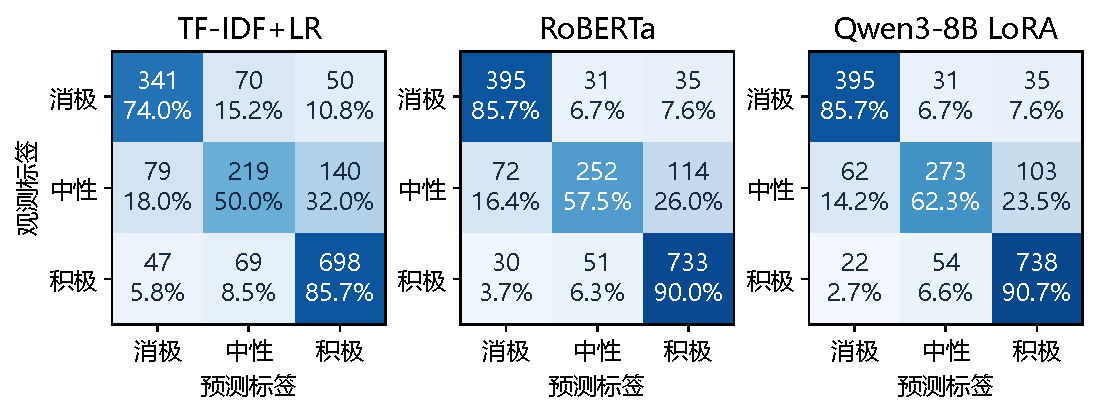
\includegraphics[width=\linewidth,height=0.80\textheight,keepaspectratio]{figures/fig_confusion.pdf}
\caption{种子 42 的混淆矩阵（计数与行内比例）}\label{fig:4-5}\end{figure}

\begin{table}[htbp]
\centering
\begin{minipage}{\textwidth}
\setlength{\tabcolsep}{3pt}
\renewcommand{\arraystretch}{1.16}
\setstretch{1.0}\fontsize{10.5}{13.5}\selectfont
\caption{种子 42 的类别指标}\label{tab:4-16}
\begin{tabular}{>{\raggedright\arraybackslash}p{\dimexpr 0.290000\linewidth-3.480000\tabcolsep\relax}>{\raggedright\arraybackslash}p{\dimexpr 0.130000\linewidth-1.560000\tabcolsep\relax}>{\raggedright\arraybackslash}p{\dimexpr 0.130000\linewidth-1.560000\tabcolsep\relax}>{\raggedright\arraybackslash}p{\dimexpr 0.150000\linewidth-1.800000\tabcolsep\relax}>{\raggedright\arraybackslash}p{\dimexpr 0.150000\linewidth-1.800000\tabcolsep\relax}>{\raggedright\arraybackslash}p{\dimexpr 0.150000\linewidth-1.800000\tabcolsep\relax}}
\toprule
\textbf{模型} & \textbf{观测类别} & \textbf{样本数} & \textbf{精确率} & \textbf{召回率} & \textbf{F1} \\
\midrule
TF-\allowbreak{}IDF+LR & 消极 & 461 & 0.730 & 0.740 & 0.735 \\
TF-\allowbreak{}IDF+LR & 中性 & 438 & 0.612 & 0.500 & 0.550 \\
TF-\allowbreak{}IDF+LR & 积极 & 814 & 0.786 & 0.857 & 0.820 \\
RoBERTa & 消极 & 461 & 0.795 & 0.857 & 0.825 \\
RoBERTa & 中性 & 438 & 0.754 & 0.575 & 0.653 \\
RoBERTa & 积极 & 814 & 0.831 & 0.900 & 0.864 \\
Qwen3-\allowbreak{}8B LoRA & 消极 & 461 & 0.825 & 0.857 & 0.840 \\
Qwen3-\allowbreak{}8B LoRA & 中性 & 438 & 0.763 & 0.623 & 0.686 \\
Qwen3-\allowbreak{}8B LoRA & 积极 & 814 & 0.842 & 0.907 & 0.873 \\
\bottomrule\end{tabular}
\par\vspace{3pt}{\fontsize{10}{12.5}\selectfont 注：所有指标直接由保存的离散预测计算；与表 4-\allowbreak{}2 的多种子均值口径不同。三个模型均以同一观测标签为参照。\par}
\end{minipage}
\end{table}

TF-IDF+LR、RoBERTa、Qwen3 LoRA 分别错误 455、333、307 条，其中涉及中性标签的错误分别为 358、268、250 条，占各自错误的 78.7\%、80.5\%、81.4\%。这里``涉及中性''指观测或预测为中性；不能把它误读为``81.4\% 的中性样本分类错误''。

Qwen3 的中性召回率为 273/438=62.3\%，高于 RoBERTa 的 252/438=57.5\%，但仍低于其消极召回率 85.7\% 与积极召回率 90.7\%。Qwen3 将 103 条中性样本判为积极、62 条判为消极，说明总体增益没有消除中性边界问题。两个模型消极行的汇总计数完全相同，不表示逐条预测也相同。

逐条配对后，Qwen3 修正了 RoBERTa 的 123 条错误，同时在 RoBERTa 正确的样本上新增 97 条错误，两者共同错误 210 条。净少错 26 条并不意味着在所有文本上单向改进；这些计数是第 4.2 节统计比较的可解释补充，而不是新的显著性证明。

\subsubsection{固定规则抽取的真实案例}

表~\ref{tab:4-17} 展示第 3.7.5 节固定抽样的六条案例，完整 12 条核读材料另存 error\_cases.csv。置信度为未温度缩放的最大类别概率，按历史文件精度保留。

\begin{table}[htbp]
\centering
\begin{minipage}{\textwidth}
\setlength{\tabcolsep}{3pt}
\renewcommand{\arraystretch}{1.16}
\setstretch{1.0}\fontsize{10.5}{13.5}\selectfont
\caption{六种误分类方向的固定抽样案例}\label{tab:4-17}
\begin{tabular}{>{\raggedright\arraybackslash}p{\dimexpr 0.080000\linewidth-0.640000\tabcolsep\relax}>{\raggedright\arraybackslash}p{\dimexpr 0.180000\linewidth-1.440000\tabcolsep\relax}>{\raggedright\arraybackslash}p{\dimexpr 0.610000\linewidth-4.880000\tabcolsep\relax}>{\raggedright\arraybackslash}p{\dimexpr 0.130000\linewidth-1.040000\tabcolsep\relax}}
\toprule
\textbf{行号} & \textbf{观测$\to$Qwen3预测} & \textbf{原始文本} & \textbf{原始置信度} \\
\midrule
300 & 消极$\to$中性 & 人民文学出版社、中华书局、商务印书馆、中华大百科,人民音乐出版社。唉可惜都不是资本喜欢的。 & 0.794 \\
324 & 消极$\to$积极 & 今天亏了4千3;不错不错;晚上吃炖好的犒劳一下自己 & 0.414 \\
921 & 中性$\to$消极 & 我就纳闷是哪个NT老师说35再买的 & 0.556 \\
1616 & 中性$\to$积极 & 这跟江铜差了7元,早知道多买点江铜了 & 0.934 \\
29 & 积极$\to$消极 & 13.15到13.50为最佳位置,工厂放假生产处与半停产状态,现在买进被套后,舂节后解放 & 0.695 \\
897 & 积极$\to$中性 & 感谢夏利.感谢张婷! & 0.559 \\
\bottomrule\end{tabular}
\par\vspace{3pt}{\fontsize{10}{12.5}\selectfont 注：行号从清洗后 test.jsonl 的第一条数据起计为 1；预测 CSV 另有一行表头。原文保留已有错字、简称及标点，箭头左侧是观测标签，不表示本文认可其为唯一正确判断。\par}
\end{minipage}
\end{table}

\textbf{局部正负线索相互冲突。} 第 324 行同时出现``亏了''与``不错不错''，存在反讽或自我宽慰的可能；Qwen3 与 RoBERTa 均判积极，而 TF-IDF 判消极。第 29 行同时有``半停产''\,``被套''和``春节后解放''的预期表达（原文为``舂节''），Qwen3 判消极，另两模型判积极。这两例说明不同模型会作出不同判断，但没有归因实验，不能声称已证明它们具体依赖了哪个词。

\textbf{观测标签与文本中的态度边界可能不一致。} 第 921 行带有``纳闷''等不满表达，观测为中性，Qwen3 判消极；另两模型为中性。第 1616 行既有价格比较，也有``早知道多买点''的反事实表达，三个模型均判积极而观测为中性，其中 Qwen3 置信度达 0.934。高置信度与模型间一致并不自动证明标签有误，这些例子更适合作为后续独立复标候选。

\textbf{短文本中的评价对象与金融语境不足。} 第 300 行列举出版社后说``唉可惜''，三个模型均判中性而观测为消极。第 897 行的``感谢''表达在缺少上下文时可能难以区分真诚赞许与其他语用，Qwen3 判中性，另两模型判积极。本文只指出可观察的文本特征，不把可能解释写成已验证机制。

以上案例按误分类方向分层，不能代表全部错误的语言类型分布，更不能计算``反讽导致多少错误''。它们与混淆矩阵共同支持的较弱结论是：中性边界、混合态度及上下文不足值得优先复核；不能由个案推出模型知识不足或标注噪声是主要原因。

\FloatBarrier\subsection{本章小结}

围绕 RQ1，LoRA 模型在本划分的三个种子中取得较高点估计，但单次配对检验经多重比较调整后不足以确证相对 RoBERTa 的稳定优势。数据曝光和清洗分析进一步说明，比较分数之前必须统一样本和处理口径。

围绕 RQ2，数据内温度交叉拟合改善了 ECE，高置信度筛选改善了子集准确率，保形方法得到接近名义目标的平均整体覆盖；三者分别回答不同问题，均不能替代独立部署验证。

围绕 RQ3，单次消融支持部分低资源配置的可行性，错误分析揭示中性类仍是主要混淆边界。概率存储精度、非独立复标、样本构成变化和缺少外部测试共同限定了本文结论的外推范围。

\clearpage\section{结论与展望}

\FloatBarrier\subsection{主要结论}

本文以中文金融社交媒体情感分类数据集 FinFE 为对象，在单张 RTX 3090 显卡上系统比较了传统机器学习、预训练语言模型和开源大语言模型三类方法，并从统计推断、置信度可靠性和数据质量三个角度对结果进行了分析。主要结论如下。

\textbf{（1）公开数据存在重复和标签冲突，应区分曝光口径并检查评估样本构成。} 原始 2020 条评估记录中有 1097 条与原始训练文件文本重叠；文件内清洗后，跨文件重叠文本为 1092 个，其中 228 个标签不同。清洗后的训练、验证和测试集规模为 8802 / 979 / 1713，集合间不存在完全重复文本。在同样的 845 条共同未曝光文本上，RoBERTa 三种子平均 F1 从未清洗训练的 0.7309 变为清洗训练的 0.7392。该比较描述清洗策略的整体差异，不识别单独的泄漏因果效应。

\textbf{（2）LoRA 微调的大模型取得了更高的分类点估计，但领先幅度有限。} 在清洗后的测试集上，TF-IDF 的宏平均 F1 约为 0.70，RoBERTa 约为 0.778，三个 LoRA 大模型为 0.798～0.807。零样本和少样本提示的 F1 约为 0.63～0.70，低于微调后的 RoBERTa。三个 LoRA 模型之间的方差分析未检出差异（p = 0.14），这不等于已证明它们等效。

\textbf{（3）模型比较应同时交代不确定性来源和多重比较口径。} 在固定数据划分的 3 个训练种子中，三个 LoRA 模型的 F1 点估计均高于 RoBERTa，Tukey 比较 p = 0.001～0.021。对种子 42 的逐条预测，McNemar 检验经 Holm 校正后不显著；50000 次配对 Bootstrap 中，三个 LoRA 对 RoBERTa 的 F1 差约为 0.018～0.019，十对比较的 Bonferroni 调整区间均包含 0。因此只能说本次重复中的点估计一致更高，尚不能证实面向新样本的稳定优势。

\textbf{（4）校准、选择性预测与集合覆盖需要分别解释。} 零样本 Qwen3 的平均置信度为 96.4\%，准确率为 67.1\%，存在明显过度自信。LoRA 模型在测试分布内五折温度交叉拟合后的 ECE 为 0.013～0.030；只回答最高置信度的 50\% 样本时准确率约为 96\%。标准保形预测整体覆盖率约为 90\%，约 77\%～78\% 的集合为单元素，但这些单元素预测的准确率仅为 88.7\%～89.3\%，不能赋予额外的 90\% 条件保证。按类别校准使中性类经验覆盖率接近 90\%，同时增加集合大小。历史概率的六位小数存储影响零样本 NLL、温度和部分并列分数，相关数值需结合截断敏感性解读。

\textbf{（5）当前消融结果提示较低资源配置可行，但不是超参数等效性证明。} 训练样本量从 500 条增加到全量时，单次 F1 从 0.766 升至 0.800；LoRA 秩 4～32 的单次 F1 为 0.798～0.809。4 比特 QLoRA 的单次 F1 为 0.807，框架记录的峰值分配显存为 11.2 GB，低于 16 位配置的 18.3 GB。由于缺少各配置的重复与等效性检验，结论限于观察到的结果，不能保证任意 12 GB 显卡环境均可运行。

\textbf{（6）重复记录揭示标签分歧，但不能据此确定性能上限。} 配对一致率为 82.9\%，按配对两端汇总边际定义的机会校正指标 K\_pair 为 0.742；82\% 的冲突涉及中性类，与中性类识别较困难的现象相一致。独立同质对称噪声模型下 q 约为 0.908，但原始文件没有独立复标证明，且清洗改变了样本构成，因此不将其解释为清洗后测试集的准确率上限，也不宣称模型已接近人工水平。

\FloatBarrier\subsection{研究不足}

本文仍存在以下不足：

（1）\textbf{只使用了一个数据集。} 本文的结论基于 FinFE 这一中文金融社交媒体数据集，是否适用于金融新闻、研究报告、上市公司公告等其他类型的文本，还需要进一步验证。

（2）\textbf{随机种子数量较少。} 受计算资源限制，每个模型只进行了 3 次独立训练，方差分析的自由度较小，对训练随机性的估计不够精确。

（3）\textbf{研究计划有所调整。} 开题时计划比较同一系列不同规模的模型（Qwen3-1.7B、4B、8B），并在 7 个样本量上各重复 3 次绘制学习曲线。实际实验中，模型比较改为三个不同系列、规模相近（7B～9B）的模型，样本量实验也只在少数几个规模上各进行了一次，因此未能系统分析模型规模的影响，学习曲线也较为粗略。

（4）\textbf{无法从重复记录识别真实标注噪声率。} q 的推算依赖给定真实类别后独立、同质和均匀错标等假设，但原始文件不提供标注者身份或金标准；重复文本也非随机样本，且清洗后测试集剔除了部分冲突记录。因此该推算仅是情景分析。

（5）\textbf{近重复和样本选择的影响尚未充分评估。} 本文只排除了规范化后的完全重复，未系统排除近重复或预训练污染；依据跨文件标签一致性删除测试记录，改变了目标人群，可能降低样本难度，不能视为原始总体的无偏随机测试样本。

（6）\textbf{错误分析尚非系统人工归因。} 本文已补充三类代表模型的混淆矩阵、类指标和固定抽样的真实案例，但未进行盲法多人编码或独立复标；因此不能估计反讽、否定、术语等错误类型的总体占比，也不能确定错误的因果来源。

（7）\textbf{概率精度和独立评估受限。} 历史预测概率只保留六位小数，丢失的尾部精度无法通过更换截断下限恢复。当前温度缩放采用测试分布内交叉拟合，保形预测也反复划分同一批样本；两者都不等同于独立外部部署验证。后续应保留高精度概率或 logits，并使用独立校准与最终评估数据。

\FloatBarrier\subsection{补充验证的优先级与触发条件}

\textbf{维持当前限定结论时，不以新增训练作为完成论文的前提。} 本文已经具备统一数据划分、五个模型的三种子训练、逐样本配对比较和可靠性分析。现有结果可以支持当前数据内的描述与条件性比较；继续增加同一测试集上的模型数量，不能补上外部效度缺口。单次消融应继续明确标为探索性，不追求通过追加种子``做出显著性''。

\textbf{若要声称对新数据稳定占优或可以部署，则需要独立测试。} 应先冻结模型、提示、清洗和阈值选择规则，再取得不参与开发的带标签文本，优先考虑不同时间或来源的同任务样本；独立校准数据与最终评估数据分开，报告类别构成、近重复检查、效应区间及人工标注过程。在反复查看过的 1713 条样本中再随机切一块，不是新的独立外部测试。样本量应依据预先设定的最小有意义效应和功效/区间精度要求确定，而不是任意指定一个整数。

\textbf{追加重复是有条件的次优先事项。} 若结论将依赖秩、量化或样本量配置之间的小差别，应对相关配置作相同种子集合下的重复，并预先确定比较家族；若要声称两种配置等效，还须预设等效界值和相应检验。当前仅说明低资源可行性，不必须把每个消融点扩展为大规模重复。更多训练种子也不能替代独立测试数据。

\textbf{高精度推理和独立复标服务于不同问题。} 若要精确比较零样本 NLL、温度或极端概率，应在固定权重下重新保存高精度概率或 logits；这属于新推理而非重新训练。若要判断中性错误主要来自标签问题，则需对预定样本开展不向标注者展示模型结果的独立复标。本文本次仅重用已有预测进行分析，未执行上述新增实验。

\FloatBarrier\subsection{研究展望}

针对上述不足，未来可以从以下几个方面继续研究：

（1）\textbf{将情感分类结果用于股价预测。} 本文得到的情感分类模型可以用于对股吧等平台的帖子进行大规模自动标注，再按个股和交易日汇总为投资者情绪指数，检验其对股票收益率、成交量和波动率的预测能力。这需要爬取帖子数据并与行情数据对齐，还需要时间顺序回测、交易成本和前视偏差控制，不能由分类分数直接推出投资收益。

（2）\textbf{扩展到更多数据和任务。} 在金融新闻、研究报告等多种文本上检验结论的普适性，并尝试细粒度的情感强度分析或面向实体的情感分析。

（3）\textbf{改进中性类的识别和标注。} 可以对中性类样本进行多人重新标注，或采用软标签、标签平滑等对噪声更稳健的训练方法，以缓解标注模糊带来的影响。

（4）\textbf{更完善的不确定性评估。} 增加随机种子数量，或采用 LoRA 集成等方法，更精确地估计训练随机性，并进一步改进大模型的校准效果。

（5）\textbf{比较不同规模的模型。} 在同一模型系列中比较不同参数规模的效果与成本，为资源受限情况下的模型选型提供更全面的参考。

\clearpage
\phantomsection\addcontentsline{toc}{section}{参考文献}
\begingroup\setstretch{1.15}\fontsize{10.5}{13}\selectfont\renewcommand{\bibfont}{\fontsize{10.5}{13}\selectfont}\setlength{\bibsep}{5pt}\begin{thebibliography}{99}
\bibitem[1]{ref1} Tetlock P C. Giving content to investor sentiment: The role of media in the stock market[J]. The Journal of Finance, 2007, 62(3): 1139-\allowbreak{}1168.

\bibitem[2]{ref2} 游家兴, 吴静. 沉默的螺旋：媒体情绪与资产误定价[J]. 经济研究, 2012, 47(7): 141-\allowbreak{}152.

\bibitem[3]{ref3} 段江娇, 刘红忠, 曾剑平. 中国股票网络论坛的信息含量分析[J]. 金融研究, 2017(10): 178-\allowbreak{}192.

\bibitem[4]{ref4} 部慧, 解峥, 李佳鸿, 吴俊杰. 基于股评的投资者情绪对股票市场的影响[J]. 管理科学学报, 2018, 21(4): 86-\allowbreak{}101.

\bibitem[5]{ref5} 沈艳, 陈赟, 黄卓. 文本大数据分析在经济学和金融学中的应用：一个文献综述[J]. 经济学(季刊), 2019, 18(4): 1153-\allowbreak{}1186.

\bibitem[6]{ref6} Loughran T, McDonald B. When is a liability not a liability? Textual analysis, dictionaries, and 10-\allowbreak{}Ks[J]. The Journal of Finance, 2011, 66(1): 35-\allowbreak{}65.

\bibitem[7]{ref7} Devlin J, Chang M W, Lee K, et al. BERT: Pre-\allowbreak{}training of deep bidirectional transformers for language understanding[C]/\allowbreak{}/\allowbreak{}Proceedings of NAACL-\allowbreak{}HLT. 2019: 4171-\allowbreak{}4186.

\bibitem[8]{ref8} Araci D. FinBERT: Financial sentiment analysis with pre-\allowbreak{}trained language models[J]. arXiv preprint arXiv:1908.10063, 2019.

\bibitem[9]{ref9} Cui Y, Che W, Liu T, et al. Pre-\allowbreak{}training with whole word masking for Chinese BERT[J]. IEEE/\allowbreak{}ACM Transactions on Audio, Speech, and Language Processing, 2021, 29: 3504-\allowbreak{}3514.

\bibitem[10]{ref10} Brown T, Mann B, Ryder N, et al. Language models are few-\allowbreak{}shot learners[C]/\allowbreak{}/\allowbreak{}Advances in Neural Information Processing Systems. 2020: 1877-\allowbreak{}1901.

\bibitem[11]{ref11} Yang A, Li A, Yang B, et al. Qwen3 technical report[J]. arXiv preprint arXiv:2505.09388, 2025.

\bibitem[12]{ref12} Wu S, Irsoy O, Lu S, et al. BloombergGPT: A large language model for finance[J]. arXiv preprint arXiv:2303.17564, 2023.

\bibitem[13]{ref13} Yang H, Liu X Y, Wang C D. FinGPT: Open-\allowbreak{}source financial large language models[J]. arXiv preprint arXiv:2306.06031, 2023.

\bibitem[14]{ref14} Hu E J, Shen Y, Wallis P, et al. LoRA: Low-\allowbreak{}rank adaptation of large language models[C]/\allowbreak{}/\allowbreak{}International Conference on Learning Representations. 2022.

\bibitem[15]{ref15} Dettmers T, Pagnoni A, Holtzman A, et al. QLoRA: Efficient finetuning of quantized LLMs[C]/\allowbreak{}/\allowbreak{}Advances in Neural Information Processing Systems. 2023.

\bibitem[16]{ref16} Zhang B, Yang H, Liu X Y. Instruct-\allowbreak{}FinGPT: Financial sentiment analysis by instruction tuning of general-\allowbreak{}purpose large language models[J]. arXiv preprint arXiv:2306.12659, 2023.

\bibitem[17]{ref17} Fatemi S, Hu Y. A comparative analysis of fine-\allowbreak{}tuned LLMs and few-\allowbreak{}shot learning of LLMs for financial sentiment analysis[J]. arXiv preprint arXiv:2312.08725, 2023.

\bibitem[18]{ref18} Paredes Amorin A, Python A, Weisser C. Fine-\allowbreak{}tuning of lightweight large language models for sentiment classification on heterogeneous financial textual data[J]. arXiv preprint arXiv:2512.00946, 2025.

\bibitem[19]{ref19} Lu D, Wu H, Liang J, et al. BBT-\allowbreak{}Fin: Comprehensive construction of Chinese financial domain pre-\allowbreak{}trained language model, corpus and benchmark[J]. arXiv preprint arXiv:2302.09432, 2023.

\bibitem[20]{ref20} Malo P, Sinha A, Korhonen P, et al. Good debt or bad debt: Detecting semantic orientations in economic texts[J]. Journal of the Association for Information Science and Technology, 2014, 65(4): 782-\allowbreak{}796.

\bibitem[21]{ref21} Dietterich T G. Approximate statistical tests for comparing supervised classification learning algorithms[J]. Neural Computation, 1998, 10(7): 1895-\allowbreak{}1923.

\bibitem[22]{ref22} Guo C, Pleiss G, Sun Y, et al. On calibration of modern neural networks[C]/\allowbreak{}/\allowbreak{}International Conference on Machine Learning. 2017: 1321-\allowbreak{}1330.

\bibitem[23]{ref23} Geifman Y, El-\allowbreak{}Yaniv R. Selective classification for deep neural networks[C]/\allowbreak{}/\allowbreak{}Advances in Neural Information Processing Systems. 2017.

\bibitem[24]{ref24} Balabanov O, Linander H. Uncertainty quantification in fine-\allowbreak{}tuned LLMs using LoRA ensembles[J]. arXiv preprint arXiv:2402.12264, 2024.

\bibitem[25]{ref25} Vaswani A, Shazeer N, Parmar N, et al. Attention is all you need[C]/\allowbreak{}/\allowbreak{}Advances in Neural Information Processing Systems. 2017: 5998-\allowbreak{}6008.

\bibitem[26]{ref26} Kaplan J, McCandlish S, Henighan T, et al. Scaling laws for neural language models[J]. arXiv preprint arXiv:2001.08361, 2020.

\bibitem[27]{ref27} McNemar Q. Note on the sampling error of the difference between correlated proportions or percentages[J]. Psychometrika, 1947, 12(2): 153-\allowbreak{}157.

\bibitem[28]{ref28} Efron B, Tibshirani R J. An introduction to the bootstrap[M]. New York: Chapman \& Hall, 1993.

\bibitem[29]{ref29} Holm S. A simple sequentially rejective multiple test procedure[J]. Scandinavian Journal of Statistics, 1979, 6(2): 65-\allowbreak{}70.

\bibitem[30]{ref30} Chow C K. On optimum recognition error and reject tradeoff[J]. IEEE Transactions on Information Theory, 1970, 16(1): 41-\allowbreak{}46.

\bibitem[31]{ref31} Vovk V, Gammerman A, Shafer G. Algorithmic learning in a random world[M]. New York: Springer, 2005.

\bibitem[32]{ref32} Angelopoulos A N, Bates S. Conformal prediction: A gentle introduction[J]. Foundations and Trends in Machine Learning, 2023, 16(4): 494-\allowbreak{}591.

\bibitem[33]{ref33} Chen W, Wang Q, Long Z, et al. DISC-\allowbreak{}FinLLM: A Chinese financial large language model based on multiple experts fine-\allowbreak{}tuning[J]. arXiv preprint arXiv:2310.15205, 2023.

\end{thebibliography}\endgroup
\end{document}
